%
% Class document definition
%
\documentclass[msc]{template/ppgccufmg}  % [phd] | [msc]



%
% Document used packages
%
\usepackage[brazil]{babel}
\usepackage[utf8]{inputenc}
\usepackage[T1]{fontenc}
\usepackage{type1ec}
\usepackage{graphicx}
\usepackage[a4paper,
      portuguese,
      bookmarks=true,
      bookmarksnumbered=true,
      linktocpage,
      colorlinks,
      citecolor=black,
      urlcolor=black,
      linkcolor=black,
      filecolor=black,
]{hyperref}
\usepackage[square]{natbib}
\usepackage{multirow}
\usepackage[usenames,dvipsnames,table,xcdraw]{xcolor} 
\usepackage{pbox}
\usepackage{multicol}
\usepackage{hyperref}
\usepackage{listings}

\hyphenation{re-qui-si-to}

\sloppy



%
% The document body and structure
%
\begin{document}



% Definitions for ppgccufmg class
\ppgccufmg{
    title={Grafos como uma primitiva do plano de controle para análise e 
        gerenciamento de Redes Definidas por Software},
    authorrev={Pantuza, Gustavo},
    cutter={M1234x}, % INFORMAÇÃO QUE VAI NA FICHA CATALOGRÁFICA
    cdu={100.0*01.10},  % Define o identificador CDU do documento, fornecido pela Secretaria do Curso.
    university={Universidade Federal de Minas Gerais},
    course={Ciência da Computação},
    address={Belo Horizonte},
    date={2015-03},
    keywords={Redes definidas por software, OpenFlow, Grafos, 
        Gerenciamento de redes, Sistemas distribuídos, Redes de computadores},
    advisor={Luiz Filipe Menezes Vieira},
    abstract=[brazil]{Resumo}{src/abstract_pt},
    abstract=[english]{Abstract}{src/abstract_en},
    %abstract=[brazil]{Resumo Estendido}{resumoest}, %resumoest.tex
    %dedication={dedicatoria},
    %ack={agradecimentos},
    %  ack=[Acknowledgments]{ack},
    epigraphtext={Live long and prosper!}{Mr. Spock},
}




% Chapters and files that compose the document content
%
% Introduction
%
\section{Introdução}


%
% Community emvolvment
%
\begin{frame}\frametitle{Apresentação}

	\begin{figure}[h]
        \centering
        
\includegraphics[scale=0.5]{images/community.png}
    \end{figure}
\end{frame}


%
% Motivation
%
\begin{frame}\frametitle{Motivação}
   
    \begin{itemize}
        \setlength{\itemsep}{1cm}
        \item A Internet demanda que a infraestrutura evolua em paralelo com 
            as aplicações e serviços
        \item Algoritmos em grafos são base para diversas aplicações em rede
        \item Computação feita em diferentes nós da rede repetidamente
        \item Logicamente centralizado, o plano de controle permite 
            minimizar a quantidade de computações
    \end{itemize}
\end{frame}


%
% Problem
%
\begin{frame}\frametitle{Problema}
    \begin{itemize}
        \setlength{\itemsep}{1cm}
        \item Uma visão topológica global é um dos principais aspectos do 
              paradigma das Redes definidas por software.
        \item Grafos representam de maneira natural e precisa a topologia 
            de uma rede.
        \item Grafos deveriam ser um recurso básico, uma premissa em 
            controladores SDN
    \end{itemize} 
\end{frame}


%
% Scientific contributions
%
\begin{frame}\frametitle{Contribuições científicas}
    \begin{itemize}
        \setlength{\itemsep}{1cm}
        \item Uma abstração da rede na forma de um grafo dinamicamente 
            atualizado.
        \item Avaliações do controlador, da rede e do protocolo OpenFlow
        \item Avaliação de grafos como primitiva em SDN
    \end{itemize}
\end{frame}


\section{Fundamentação teórica}

\section{SDN}



%
% SDN
%
\begin{frame}\frametitle{SDN}

    \begin{itemize}
    \item SDN é apenas um modelo
    \vspace*{0.5cm}
    \item Um \emph{design} para construção e administração de redes
    \vspace*{0.5cm}
    \item A separação dos planos de controle e de dados torna o 
          funcionamento da rede mais flexível
    \end{itemize}
\end{frame}

%
% SDN
%
\begin{frame}\frametitle{Características}

    \begin{itemize}
    \item Torna a rede programável
    \vspace*{0.1cm}
    \item Flexibilidade na administração da rede
    \vspace*{0.1cm}
    \item Controle logicamente centralizado
    \vspace*{0.1cm}
    \item Configurável via programação
    \vspace*{0.1cm}
    \item Padronização aberta 
    \end{itemize}
\end{frame}


%
% Openflow
%
\begin{frame}\frametitle{Openflow}

    \begin{itemize}
    \item Se SDN é só um modelo, como implementá-lo?
    \end{itemize}
    	\begin{figure}[h]
        \centering
        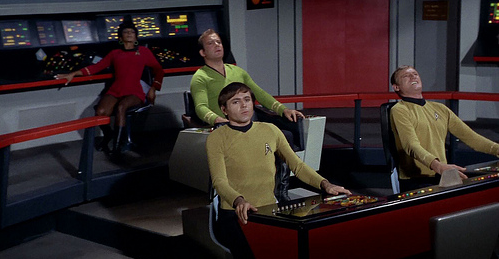
\includegraphics[scale=0.5]{images/control-room.png}
    \end{figure}
\end{frame}



%
% Openflow
%
\begin{frame}\frametitle{Openflow}

    \begin{itemize}
    \item Openflow é um protocolo que possibilita experimentos e aplicações
          em SDN
    \end{itemize}
    	\begin{figure}[h]
        \centering
        
\includegraphics[scale=0.3]{images/openflow.png}
    \end{figure}
\end{frame}


%
% Openflow
%
\begin{frame}\frametitle{Openflow}

    \begin{itemize}
    \item \href{http://archive.openflow.org/documents/openflow-wp-latest.pdf}{Artigo} publicado em 2008 
    \item Permitiu que pesquisadores pudessem criar experimentos com novos
          protocolos em redes convencionais 
    \end{itemize}

\end{frame}




%
% Openflow
%
\begin{frame}\frametitle{Porque é tão importante?}

    \begin{itemize}
    \item A arquitetura da Internet tem deficiências
    \item Inovações em rede custam caro
    \item A arquitetura continua acoplada à infraestrutura
    \item O Openflow define um padrão que qualquer fabricante de     
          \emph{hardware} de rede pode implementar
    \end{itemize}

\end{frame}


\subsection{O protocolo OpenFlow}


%
% Openflow
%
\begin{frame}\frametitle{Openflow}

    \begin{itemize}
    \item Openflow é um protocolo que possibilita experimentos e aplicações
          em SDN
    \end{itemize}
    \begin{figure}[h]
        \centering
        
\includegraphics[scale=0.2]{images/openflow}
    \end{figure}
\end{frame}


%
% Openflow
%
\begin{frame}\frametitle{Openflow}

    \begin{itemize}
        \setlength{\itemsep}{.5cm}
    \item \href{http://archive.openflow.org/documents/openflow-wp-latest.pdf}
        {OpenFlow: Enabling Innovation in Campus Networks} publicado em 2008 
    \item Permitiu que pesquisadores criassem experimentos com novos
          protocolos em redes convencionais.
    \end{itemize}

\end{frame}




%
% Openflow
%
\begin{frame}\frametitle{Definição}

    \begin{itemize}
        \setlength{\itemsep}{.5cm}
        \item Consiste em uma interface de programação para o \emph{switch}
        \item A interface separa de maneira clara os planos de dados e de 
            controle
        \item Um programador pode, através de um programa, controlar a
            forma como um \emph{switch} executa seu encaminhamento de pacotes
        \item O OpenFlow foi criado como um padrão aberto
    \end{itemize}
\end{frame}


%
% Openflow
%
\begin{frame}\frametitle{Componentes}
    Na arquitetura estabelecida pelo protocolo OpenFlow existem dois papéis
    principais.

    \begin{figure}[h]
        \centering
        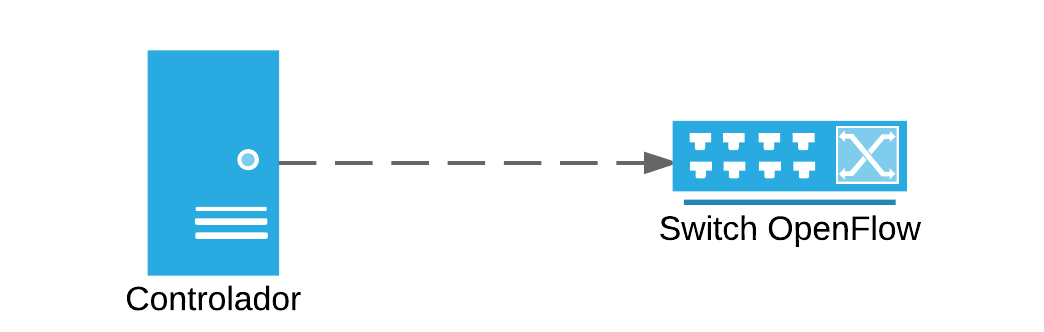
\includegraphics{images/controller-secure-switch}
        \caption{Da esquerda pra direita, plano de controle e plano de dados}
    \end{figure}

\end{frame}


%
% Openflow
%
\begin{frame}\frametitle{Arquitetura OpenFlow}

    \begin{figure}[h!]
        \centering
        \label{fig:switch-arch}
        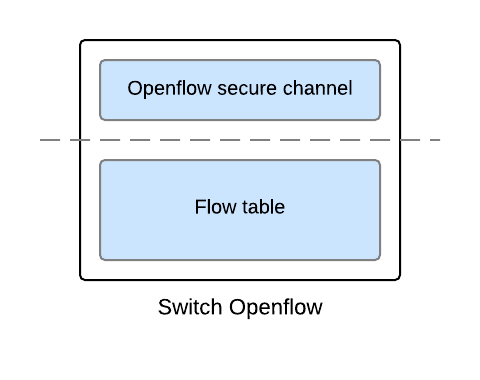
\includegraphics[width=\linewidth]{images/switch-architecture}
        \caption{Arquitetura do comutador OpenFlow}
    \end{figure}

\end{frame}



%
% Switch Archtecture
%
\begin{frame}\frametitle{Arquitetura Openflow}

    \begin{itemize}
        \setlength{\itemsep}{.5cm}
    \item \textbf{Canal seguro OpenFlow}: É a conexão segura entre o
          controlador e o switch openflow
    \item \textbf{Tabela de fluxos}: É a tabela onde são identificados os fluxos
    \item Para cada fluxo tem-se uma ação (action) a ser tomada
    \end{itemize}
\end{frame}


%
% Switch Archtecture
%
\begin{frame}\frametitle{Tabela de fluxos}
    \begin{table}[h!]
    \small
    \centering
    \begin{tabular}{ | l | l | l | l |}
    \hline
    \textbf{Cabeçalho} & \textbf{Contadores} & \textbf{Ações} &
    \textbf{Prioridade} 
    \\ \hline porta de ingresso=5 & 55635 bytes & \pbox{20cm}{Encaminhar 
    \\ porta=8} 
    & 100 \\ \hline
    \pbox{20cm}{Endereço ip=192.168.1.42 \\ porta=80} & 4032 bytes &
    \pbox{30cm}{Rescrita \\ ip=192.168.1.100} & 500 \\ 
    \hline Protocolo IP=UDP & 100 bytes 
    & Drop & 700 \\ \hline
    \end{tabular}
    \caption{Tabela de fluxos simplificada}
    \label{tbl:flowtable}
\end{table}

\end{frame}

%
% Switch Archtecture
%
\begin{frame}\frametitle{Cabeçalho OpenFlow}

    \begin{itemize}
    \item Um fluxo é identificado pelos seguintes campos do cabeçalho 
          Openflow:
    \end{itemize}
	\begin{figure}[h]\hspace*{-1.2cm}
        \centering
        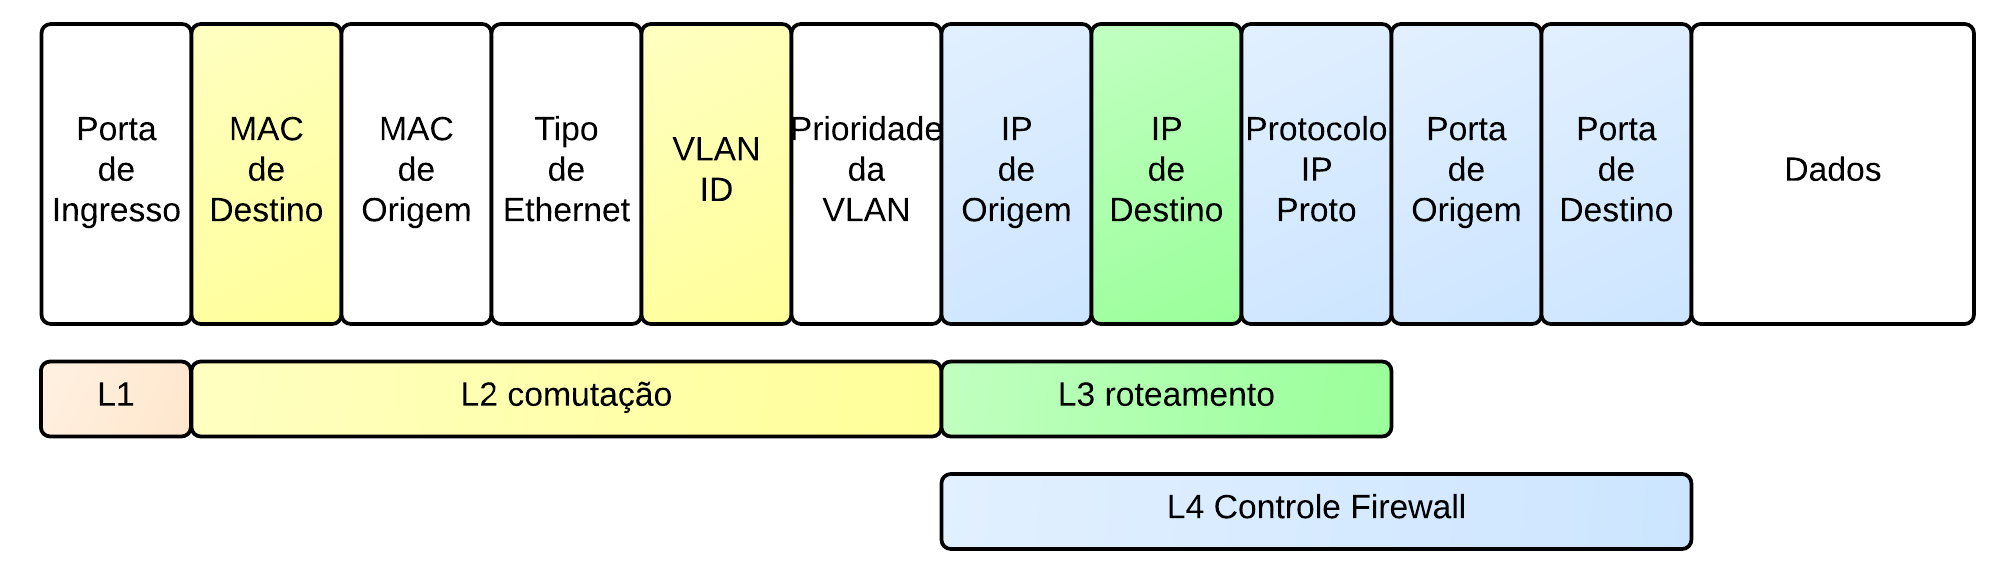
\includegraphics[width=\linewidth]{images/openflow-header}
    \end{figure}
\end{frame}



%
% Actions
%
\begin{frame}\frametitle{Ações}

	\begin{figure}[h]
        \centering
        
\includegraphics[scale=0.5]{images/action.png}
    \end{figure}
    
\end{frame}


%
% Actions
%
\begin{frame}\frametitle{Tipos de ações}

    \begin{columns}[T] % align columns
        \begin{column}{.33\textwidth}

            \begin{itemize}
                \item Forwarding
                \item Drop
                \item Set
                \item strip
                \item Copy-in
                \item Copy-out
                \item Push
                \item Pop
                \item Dec
            \end{itemize}
        \end{column}%
        \hfill%
        \begin{column}{.67\textwidth}
            \begin{figure}[!htb]
                \centering
                
\includegraphics[scale=0.5]{images/action-types}
            \end{figure}
        \end{column}%
    \end{columns}

\end{frame}


%
% Controller
%
\begin{frame}\frametitle{Controlador}

    \begin{itemize}
        \setlength{\itemsep}{.5cm}
    \item É um software que se conecta de maneira segura ao switch openflow
          com o objetivo de manipular sua tabela de fluxos
    \item Esse software pode ser distribuído
    \item Ele representa uma entidade lógica e centralizada
    \item Permite que outros programas troquem mensagens com o 
        plano de controle da rede
    \item Pode calcular estatísticas da rede
    \end{itemize}

\end{frame}


%
% Controller
%
\begin{frame}\frametitle{Controlador}

    \begin{itemize}
    \item Cabe ao programador lidar com os problemas típicos em 
          desenvolvimento de software:
          \begin{itemize}
          \item Tolerância a falha
          \item Persistência
          \item Eficiência
          \item Projeto/design de implementação
          \item debugging
          \item Testes
          \end{itemize}
    \end{itemize}
\end{frame}


%
% Controller
%
\begin{frame}\frametitle{Controlador}

    \begin{itemize}
    \item Controladores Openflow:
          \begin{itemize}
          \item Biblioteca \href{http://opennetworkingfoundation.github.io/libfluid/index.html}{Libfluid}
                para criação de aplicações/controladores em SDN
          \item \href{http://www.noxrepo.org/nox/about-nox/}{Nox Controller}
          \item \href{https://openflow.stanford.edu/display/Beacon/Home}{Beacon}
          \item \href{http://www.noxrepo.org/pox/about-pox/}{Pox Controller}
          \item \href{http://osrg.github.io/ryu/}{Ryu}
          \end{itemize}
    \end{itemize}
\end{frame}

\section{architecture}


%
% Archtecture
%
\begin{frame}\frametitle{Arquitetura Openflow}

    \begin{itemize}
    \item Temos dois papeis principais:
        \begin{itemize}
        \item Controlador
        \item Switch Openflow
        \end{itemize}
    \item Algo te lembra plano de dados e controle desacoplados?
    \end{itemize}
    
	\begin{figure}[h]
        \centering
        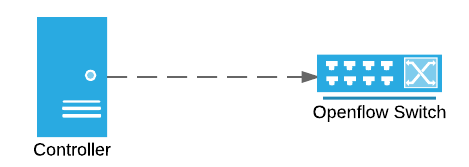
\includegraphics[scale=0.6]{images/controller-to-openflow.png}
    \end{figure}
\end{frame}



%
% Switch Archtecture
%
\begin{frame}\frametitle{Arquitetura do Switch Openflow}

    \begin{itemize}
    \item Internamente um Switch openflow é assim:
    \end{itemize}
    
	\begin{figure}[h]
        \centering
        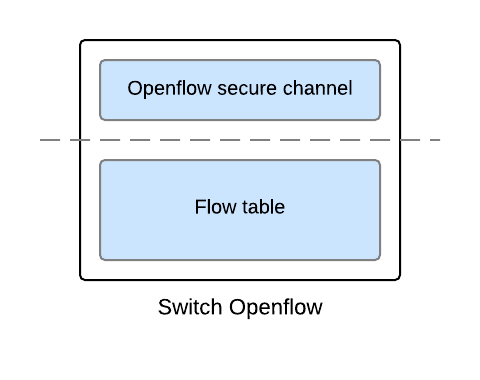
\includegraphics[scale=0.5]{images/openflow-switch-architecture.png}
    \end{figure}
\end{frame}

%
% Switch Archtecture
%
\begin{frame}\frametitle{Arquitetura Openflow}

    \begin{itemize}
    \item \textbf{Openflow secure channel}: É a conexão segura entre o
          controlador e o switch openflow
    \vspace*{0.5cm}
    \item \textbf{Flow table}: É a tabela onde são identificados os fluxos
    \vspace*{0.5cm}
    \item Para cada fluxo tem-se uma ação (action) a ser tomada
    \end{itemize}
\end{frame}

%
% Switch Archtecture
%
\begin{frame}\frametitle{Arquitetura Openflow}

    \begin{itemize}
    \item Um fluxo é identificado pelos seguintes campos do cabeçalho 
          Openflow:
    \end{itemize}
	\begin{figure}[h]\hspace*{-1.2cm}
        \centering
        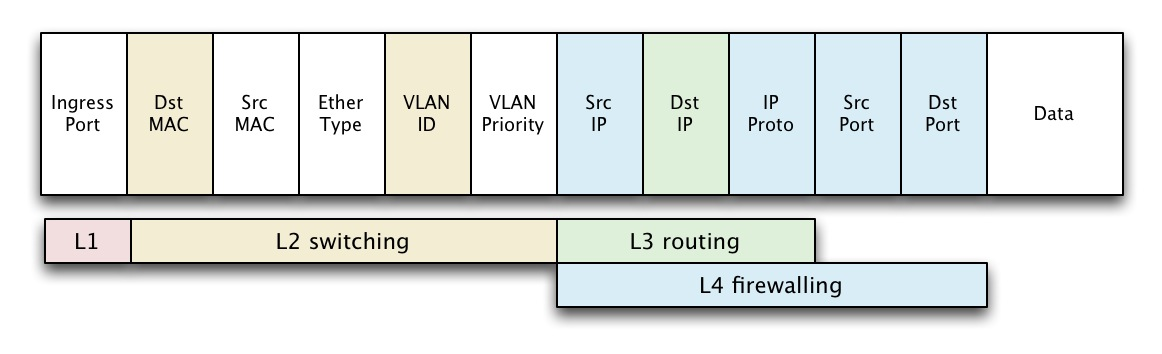
\includegraphics[scale=0.32]{images/openflow-header.jpg}
    \end{figure}
    
\end{frame}


%
% Actions
%
\begin{frame}\frametitle{Actions}

	\begin{figure}[h]
        \centering
        
\includegraphics[scale=0.5]{images/action.png}
    \end{figure}
    
\end{frame}


%
% Actions
%
\begin{frame}\frametitle{Tipos de Actions}

    \begin{itemize}
    \item Forwarding
    \item Drop
    \item Set
    \item strip
    \item Copy-in
    \item Copy-out
    \item Push
    \item Pop
    \item Dec
    \end{itemize}

\end{frame}


%
% Flow table 
%
\begin{frame}\frametitle{Tabela de Fluxos}

\begin{center}
    \begin{tabular}{ | l | l | l | l |}
    \hline
    \textbf{Header} & \textbf{Counters} & \textbf{Actions} & \textbf{Priority} \\ \hline
    in\_port=5 & 55635 bytes & \pbox{20cm}{Forward \\ port=8} & 100 \\ \hline
    \pbox{20cm}{ip=192.168.1.42 \\ port=80} & 4032 bytes & \pbox{30cm}{Set \\ rewrite \\ ip=192.168.1.100} & 500 \\ \hline
    ipproto=UDP & 100 bytes & Drop & 700 \\ \hline
    \end{tabular}
\end{center}

\end{frame}

%
% Controller
%
\begin{frame}\frametitle{Controlador}

    \begin{itemize}
    \item É um software que se conecta de maneira segura ao switch openflow
          com o objetivo de manipular sua tabela de fluxos
    \item Esse software pode ser distribuído
    \item Ele representa uma entidade lógica e centralizada
    \item É possível ter visão e controle de estado global da rede
    \item Permite que outros serviços e programas façam requisições e troca
          de mensagem com o plano de controle da rede
    \item Pode calcular estatísticas da rede
    
    \end{itemize}

\end{frame}


%
% Controller
%
\begin{frame}\frametitle{Controlador}

    \begin{itemize}
    \item Cabe ao programador lidar com os problemas típicos em 
          desenvolvimento de software:
          \begin{itemize}
          \item Tolerância a falha
          \item Persistência
          \item Eficiência
          \item design de implementação
          \item debugging
          \item Testes
          \end{itemize}
    \end{itemize}
\end{frame}

%
% Controller
%
\begin{frame}\frametitle{Controlador}

    \begin{itemize}
    \item Controladores Openflow:
          \begin{itemize}
          \item Biblioteca \href{http://opennetworkingfoundation.github.io/libfluid/index.html}{Libfluid}
                para criação de aplicações/controladores em SDN
          \item \href{http://www.noxrepo.org/nox/about-nox/}{Nox Controller}
          \item \href{https://openflow.stanford.edu/display/Beacon/Home}{Beacon}
          \item \href{http://www.noxrepo.org/pox/about-pox/}{Pox Controller}
          \item \href{http://osrg.github.io/ryu/}{Ryu}
          \end{itemize}
    \end{itemize}
\end{frame}


%
% Simple topology
%
\begin{frame}\frametitle{Arquitetura Openflow}

    \begin{itemize}
    \item Uma topologia simples:
    \end{itemize}
    
	\begin{figure}[h]
        \centering
        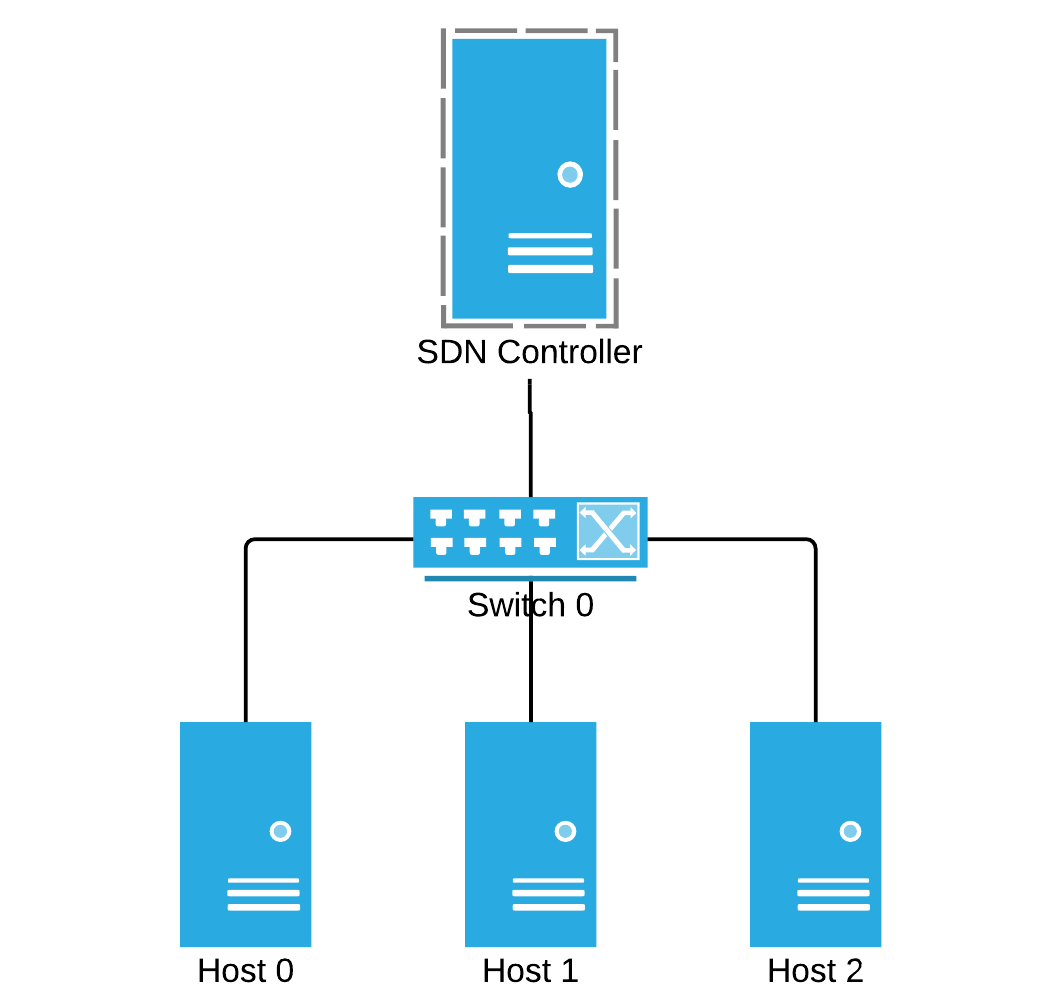
\includegraphics[scale=0.3]{images/simple-topology.png}
    \end{figure}
\end{frame}


%
% N openflow 
%
\begin{frame}\frametitle{Arquitetura Openflow}

    \begin{itemize}
    \item Um controlador para vários \emph{Switches}
    \end{itemize}
    
	\begin{figure}[h]
        \centering
        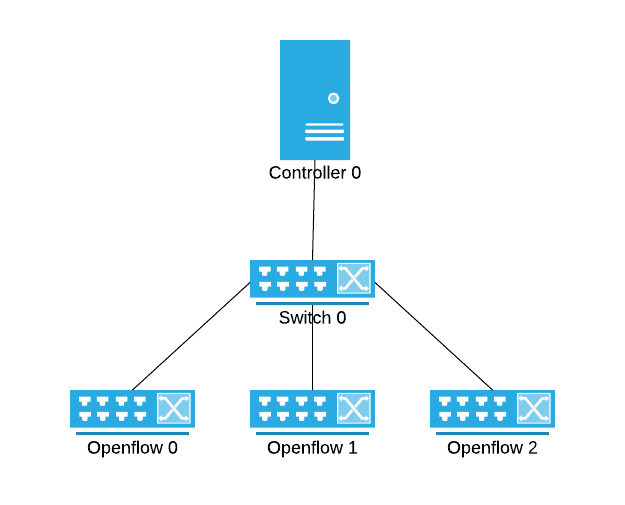
\includegraphics[scale=0.4]{images/n-openflow-switches.png}
    \end{figure}
\end{frame}


%
% SDN inter domain
%
\begin{frame}\frametitle{Arquitetura Openflow}

    \begin{itemize}
    \item Comunicação entre domínios de rede
    \end{itemize}
    
   
	\begin{figure}[h]\hspace*{-1cm}
        \centering
        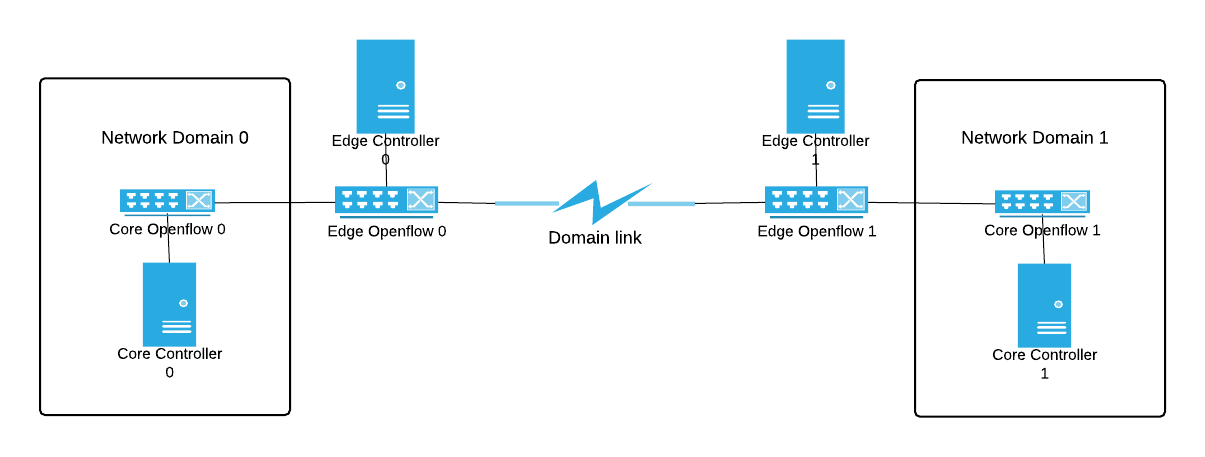
\includegraphics[scale=0.3]{images/edge-core-sdn.png}
    \end{figure}
\end{frame}



%
% Distributed openflow controller
%
\begin{frame}\frametitle{Arquitetura Openflow}

    \begin{itemize}
    \item Controlador distribuído
    \end{itemize}
    
	\begin{figure}[h]
        \centering
        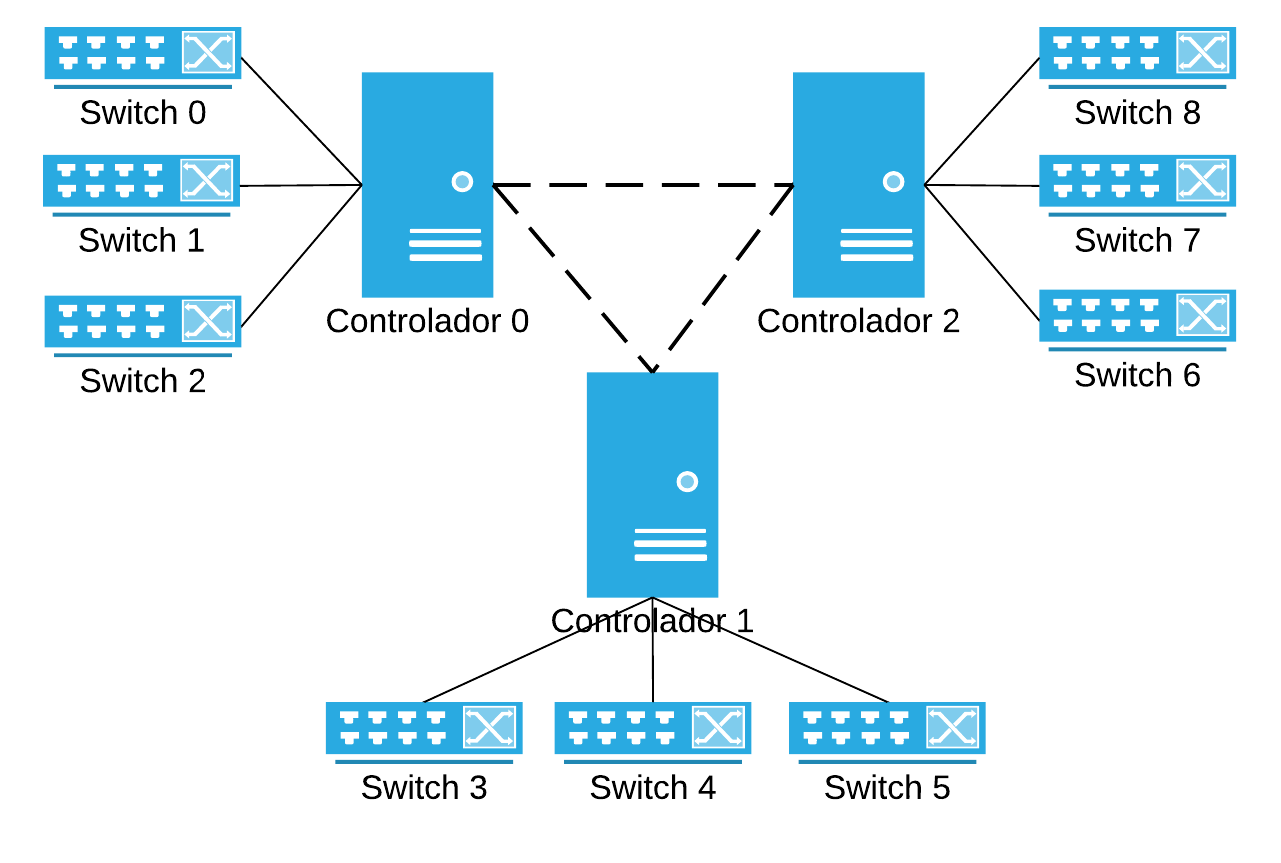
\includegraphics[scale=0.4]{images/distributed_sdn_controller.png}
    \end{figure}
\end{frame}

\chapter{Trabalhos relacionados}

Essa seção apresenta os trabalhos relacionados ao presente projeto de 
dissertação e discute suas características.
A seção segue uma linha cronológica com temas e artigos que levam a 
formulação que é a base do presente trabalho.

\section{As redes em camadas (\emph{Overlay})}

Um entendimento das implicações de redes \emph{overlays} para a 
arquitetura da Internet, para o mercado e para a política
é apresentado em \citep{clark2006overlay}. 
De modo geral o artigo descreve, principalmente, as redes de 
CDN (Redes de entrega de conteúdo), segurança e roteamento em camadas. 
O artigo posiciona as \emph{overlays} como uma uma camada intermediária, 
acima dos protocolos básicos IP e abaixo da camada de 
aplicação. 
Segundo essa visão, \emph{overlays} são para a internet básica (ponto-a-ponto)
usuários finais em que, por exemplo, um roteador apenas encaminha pacotes sem
se importar com seu conteúdo ou finalidade. 
Por outro lado, para a aplicação ela se comporta como sua infraestrutura. 
Segundo o autor, as \emph{overlays} se tornaram o principal meio de 
evolução da arquitetura da Internet.

Utilizar \emph{overlay} para tratar as deficiências da rede é custoso, no
entanto atualizar a infraestrutura da Internet básica seria ainda mais. 
As redes \emph{overlays} irão, de maneira disruptiva, representar o modo de 
inovar dentro da Internet criando novos jogadores, 
um novo cenário econômico e novas regras.

A arquitetura RON (\emph{Resilient Overlay Network}) 
\citep{anderson2001resilient} é capaz de tornar a entrega de pacotes na 
Internet mais confiável através de detecção e recuperação de interrupções e 
falhas no roteamento. 
A Internet foi criada como uma rede \emph{overlay} que funcionava sobre a rede 
de telefonia. Ou seja, o conceito de Redes \emph{overlay} não é uma idéia nova.
No entanto, poucas dessas redes foram estruturadas para se recuperar e tolerar 
falhas de forma eficiente. Nesse contexto é que as RONs demonstram ser 
confiáveis.

As RONs possuem três Metas/objetivos. O primeiro objetivo e principal é 
permitir que um grupo de nós possam se comunicar independente de haver uma 
falha na rota entre eles. 
Isso torna o roteamente confiável. O segundo objetivo
é tornar o roteamento e a seleção de próximo host com aplicações distribuídas 
mais forte, mais eficiente do que tradicionalmente é feito com outras 
arquiteturas e protocolos. 
O terceiro e último objetivo é fornecer um framework 
para implementação de políticas de roteamento que governam a escolha de rotas 
dentro da rede. 

As implicações de desempenho entre a rede \emph{overlay} Gnutella e a 
infra-estrutura da Internet é descrito em \citep{ripeanu2002mapping}. 
Redes P2P agregam vários computadores que entram e saem da rede todo o tempo. 
Esses Peers (computadores) podem não ter um endereço IP permanente. 
As redes P2P são entidades independentes e auto organizadas. 
Esse trabalho descreve um período de avaliação de sete meses do crescimento das 
redes Gnutella assim como suas implicações de desempenho. 
A rede é composta por serventes (computadores) que são os nós da rede virtual 
na camada de aplicação em que seus enlaces são formados por conexões 
TCPs abertas. 
Ao analisar a topologia utilizada pelo Gnutella o artigo explicita que apesar 
de essas redes serem eficientes em lidar com falhas aleatórias em computadores,
elas estão vulneráveis a ataques bem planejados.

\section{Redes centradas em conteúdo}

\emph{Content-Centric Networking} (CCN, redes centradas no conteúdo) trata o 
conteúdo como uma primitiva\citep{van2009networking}. 
Esse conteúdo é requisitado através de um nome. 
Em analogia ao IP, a CCN substitui o 'onde', utilizado no IP, pelo 'o que'. 
A comunicação dentro da CCN é definida por 'consumidores de dados'. 
Existem dois tipos de pacotes: \emph{Interest} (interesse) 
e \emph{Data} (dado).    

O documento descreve o funcionamento completo do roteamento dos pacotes 
baseados em conteúdo, assim como seria seu comportamento dentro de 
intra-domínios e inter-domínios. 
A segurança acontece no nível do dado ao invés de apenas uma propriedade da 
conexão pela qual o dado trafega. 
O projeto de CCN's a protege de várias classes de ataques de rede. 
O artigo apresenta comparações e avaliações de CCN's em relação ao TCP/IP. 
São relacionados temas como eficiência na tranferência de dados, 
eficiência na distribuição de conteúdo, a estratégia de camadas da rede 
e voz sobre CCN. 
A CCN foi projetada para substituir o IP, mas pode ser distribuída 
como um overlay. 

O artigo \citep{dilley2002globally} apresenta como o CDN 
(\emph{Content Delivery Network}) da Akamai's lidou com gargalos e falhas 
através de servidores de borda. 
Esses servidores são responsáveis por aliviar o serviço de estressar um único 
servidor. 
Servir conteúdo na \emph{Web} com apenas um servidor são sérios problemas 
para escalabilidade, confiança e performance de um sítio/serviço.

Ao estabelecer servidores de borda que possuem tarefas específicas, 
é necessário tratar suas falhas individulamente.
Em função dessas características, o artigo apresenta soluções com servidores de
borda através da utilização de aproximação (proxy), provisionamento (caches), 
replicação, sincronia, balanceamento de carga, tolerância a falhas, 
autenticação, segurança, recuperação de erros e monitoramento de serviços. 
O artigo propôe que o grande desafio para lidar com esses circunstâncias é 
identificar os design patterns (padrões de desenho/implementação) que são 
soluções de custo efetivo e úteis ao sistema de maneira global.


Uma experiência relevante foi a utilização do CoralCDN durante seus cinco
anos de deploy (publicação).
Com o enorme crescimento em utilizar virtualização e deploy em cloud, 
os serviços na Internet estão cada vez mais descentralizando
sua infra-estrutura. 
O CoralCDN foi desenvolvido de maneira escalável e automática para lidar com 
picos repentinos no tráfego de conteúdo \citep{freedman2010experiences}. 
O artigo demonstra a sequência de acontecimentos que ocorrem dentro da rede de 
aproximadores (proxys), servidores de índice, DNS e origem quando um cliente 
requisita uma url ao CDN. 

O CoralCDN, objetiva poupar ao máximo os servidores origem. 
A utilização de aproximadores (proxys) e provisionamento (cache) 
garantem que esse objetivo seja cumprido. 
O funcinamento interno do CDN estabelece políticas de acesso aos conteúdos. 
Diferenciando políticas para recuperar conteúdos antigos, conteúdos não 
populares, excessos para conteúdos populares e de muito acesso. O CDN 
disponibiliza também, uma API aberta para permitir elasticidade na 
distribuição de conteúdo. 

O protocolo Chord de pesquisa de itens em nós dentro de uma 
rede Peer-to-peer é aprensentado em \citep{ion2001chord}. 
O Chord executa apenas uma operação em que, dada uma chave, 
ele mapeia a chave a um nó (host). 
A tabela de roteamento Chord é distribuída e utiliza hashing para 
atribuir uma chave a um nó. 
O artigo prova que a complexidade algorítmica dessa busca é O(log N).
O Chord simplifica o modelo P2P, lidando apenas com balanceamento de carga, 
descentralização, escalabilidade, disponibilidade e nomeação flexível. 
É provado que as buscas recursivas são mais eficientes em 
função do tempo de execução do que as pesquisas iterativas. 
Diferentemente de P2Ps como Napster e Gnutella, o protocolo Chord melhora a 
escalabilidade da tarefa de embaralhamento (hashing), pois ele evita que 
todos os nós tenham que saber sobre todos os demais nós. 

ICN (Information Centric Network) \citep{bong2009information} é uma abordagem 
parecida com a CCN (Content centric Network). 
O artigo mostra uma arquitetura bem parecida com SDNs onde o plano de controle 
está separado do plano de dados. Mostra também que esses planos são unidades 
lógicas dentro da rede. Ou seja, o controlador pode ser composto por diversos 
equipamentos (entidades) na rede. 

O artigo, abstrai o funcionamento da busca de dados dentro da rede. 
Ele parte do pressuposto que a busca funcione como um DNS, dado que a busca é 
feita por pacotes que carregam os interesses de quem iniciou a requisição. 
Os switches ao longo da rede fazem cache dos pacotes de dado, podendo 
responder a requisição sozinhos. 

\section{O protocolo OpenFlow e as inovações em rede}

A evolução da Internet é uma discussão polêmica. 
O artigo \citep{jennifer2010future} apresenta dois pontos de vista.
O primeiro defende que a Internet necessita de um redesign. 
O segundo apresenta um ponto de vista contrário argumentando que a rede 
deve evoluir e não ser recontruída.

O primeiro ponto de vista levanta questionamentos como se deve-se continuar
fazendo melhorias na rede ou se contruir uma nova arquitetura seria melhor, 
dado que elas seriam irrestritas pelo atual modelo. 
É argumentado que o sucesso da atual Internet não significa que 
ela está amadurecida. 
É descrito que a rede não está preparada para os dispositivos e 
pequenos sensores, atualmente utilizados dentro da rede, que podem 
revolucionar a sociedade contemporânea.

Um contraponto é apresentado dizendo que a economia industrial moderna não 
está habilitada a receber essas tecnologias emergentes e que isso involveria 
custos inconscebíveis em mudar operação e tecnologia envolvida. 
É descrito também que os estudos de novas arquiteturas para a rede, para que 
seja aceitável, deve substituir por completo o atual modelo. 
Do contrário, seria apenas mais exercício intelectual para a contrução 
da nova rede. 

O projeto do protocolo OpenFlow foi apresentado em \citep{nick2008openflow}. 
Ele é uma forma de pesquisadores experimentarem novos protocolos nas redes 
utilizadas no dia-a-dia. Ele é baseado nos switches ethernet com uma tabela de 
fluxos e uma interface bem definida de comunicação com computadores externos. 

Os pesquisadores podem controlar seus próprios fluxos, escolhendo uma rota
alternativa para os pacotes ou executando algum processamento no pacote. 
Eles podem testar modelos de segurança, schemas de endereçamento e até 
alternativas ao protocolo IP. 
É possível fazer estudos em redes isoladas, em administração de redes, 
em controle de acesso, autenticação e processamento de pacotes.
O OpenFlow possibilita experimentações de maneira uniforme em switches 
completamente heterogeneos. 

Baseando-se em SDN, o artigo \citep{barath2012software} propõe uma arquitetura 
na linha evolucionária para Internet.
Como a arquitetura da Internet possui deficiências e possui diversos fatores
que impedem que ela seja substituída, o artigo traz uma abordagem que dissocia 
a infraestrutura da arquitetura da Internet. 

A arquitetura proposta envolve fundamentos trazidos de SDN, MPLS e 
encamimhamento via programas (\emph{software forwarding}). 
Nessa arquitetura, as redes seriam domínios. 
Cada domínio possui um controlador do núcleo (\emph{core}) e um 
de borda (\emph{edge}). 
Os controladores de borda controlam o tráfego externo. 
Os de núcleo controlam o interior dos domínios. 
Isso cria uma camada de isolamento em que pode-se alterar protocolos e 
algorítmos em ambos os ambientes, núcleo e borda, sem que um interfira 
no outro.
Além disso foram mostrados modelos de serviços que podem ser estruturados 
sobre essa arquitetura. 
O artigo apresenta três exemplos de sistemas de redes que poderiam funcionar 
perfeitamente sobre essa arquitetura.

\section{Computação em arquiteturas na nuvem (\emph{cloud})}

O artigo \citep{arsalan2009applying} apresenta o NOX 
(\emph{Networking Operanting System}). 
O NOX traz um controle lógico centralizado de alto nível de abstrações de 
rede como usuários, topologia, serviços e controle da rede. 
Através do OpenFlow ele adiciona entradas de fluxo (\emph{flow entries}) na 
tabela de encaminhamento dos switches. 

O projeto permite implementações em C++ e Python. 
A abordagem do artigo é voltada para datacenters. 
São demonstradas interações com PortLand e LV2. 
O grande objetivo desse sistema de gerenciamento é prover um controle da rede,
flexível suficiente, para atender uma ampla gama de necessidades de rede em 
datacenters. 
Pelo fato de artigo trazer uma abordagem mais comercial (\emph{datacenters}), 
são demonstradas as necessidades e problemas enfrentados por 
\emph{datacenters} e como o NOX demonstra-se uma ferramenta que flexibiliza 
e facilita o design dessas aplicações comerciais.

Visando solucionar o problema de migração de máquinas virtuais, 
o artigo \citep{erik2012live} apresentao LIME.
Ele é uma solução baseada em SDN que isola a aplicação da topologia da rede e 
de como ela é controlada. 
A proposta visa reduzir o tempo com que a migração e sincronia acontecem.

Ao iniciar uma migração de máquina virtual, os switches que estavam no local 
de origem e os do local de destino são agrupados em um único switch virtual. 
Todo o fluxo de dados é repassado ao controlador SDN que controla todo o 
tráfego durante o processo de migração. 
Concluída a migração o LIME reprograma os switches e descarta a necessidade 
do controlador SDN interferir no trafego.

Os dispositivos intermediários (\emph{middleboxes}) são parte crucial das 
grandes redes comporativas, centros de dados 
(\emph{datacenters}) e computação na nuvem (\emph{clouds}). 
Seu gerenciamento é complexo dinâmico.
O artigo \citep{aaron2012toward} apresenta a idéia de um arcabouço 
(\emph{framework}) utilizando SDN para gerenciar os dispositivos 
\emph{middleboxes}. 

O trabalho apresenta um arcabouço (\emph{framework}) que possibilita 
novas aplicações.
Com a separação do plano de dados do plano de controle através da SDN, 
tem-se maior flexibilidade para posicionar os dispositivos (\emph{middleboxes})
dentro da rede, assim como simplificar seu gerenciamento. 
São apresentados também abstrações e interfaces para lidar
com os estados dos dispositivos intermediários (\emph{middleboxes}). 
Essa tarefa não é nada trivial, pois esses dispositivos (\emph{middleboxes}) 
podem ser muito diferentes uns dos outros.

A configuração em tempo real (\emph{run-time}) de redes para 
grandes volumes de dados (\emph{big data}) com o objetivo de otimizar a 
aplicação juntamente com o desempenho e utilização da rede é apresentado
em \citep{programming2012guohui}.
O trabalho se baseia na utilização de \emph{switches} óticos como premissa 
para aumentar a performance.
A abordagem dos autores envolve um controlador SDN que é uma 
interface para as aplicações dentro do datacenter. 
O artigo foca bastante na topologia física e no roteamento de 
aplicações em \emph{big data}.
Ao utilizar um controlador SDN, as aplicações em \emph{big data} tornam-se 
mais próximas à rede que está abaixo da aplicação. 
O artigo utiliza o \emph{Hadoop} como exemplo de testes. São discutidos 
aspectos de integração de rede, agendamento de tarefas, topologia e 
configuração de rotas para processos \emph{Hadoop}. 


\section{Recuperação de informação topológica}

A necessidade de se buscar e monitorar dados 
específicos, principalmente em redes complexas, atrai o desenvolvimento
de linguagens DSL (linguagens de domínio especifico) que simplifique, 
organize, generalize e garanta eficiência na manipulação desses dados.
Esse é o exemplo do Frenetic \citep{foster2011frenetic} 
e do Pyretic \citep{monsanto2013composing}.

O Pyretic introduz novas abstrações para criação de aplicações de vários
módulos independentes, que em juntos administram o tráfego e 
abstraem a topologia da rede. 
O sistema utiliza uma linguagem chamada Pyretic \citep{monsanto2013composing}. 
O sistema funciona em cima do POX. 
Ele converte regras de plano de controle programadas em Pyretc para o plano 
de dados dos dispositivos de rede dentro de um SDN. 
O artigo apresenta o conjunto de regras de composição como regras de ação, 
regras de predicado, regras de consulta, etc. 
O Pyretic é uma linguagem que permite programadores a criarem grandes e 
sofisticadas aplicações SDN com pequenos módulos independentes. 

Enquanto a abordagem da DSL é baseada em atuação, execução,
conjunta com o controlador,
o NIB é baseada em um banco de dados distribuído,
com uma abordagem mais ampla e atacando problemas mais gerais
como persistência, concorrência, redundância, escalabilidade, etc.

\section{A abordagem em grafos}

A abordagem de representar a rede na forma de um grafo foi mencionada 
por Casado \emph{et al.} em um dos primeiros artigos sobre SDN
\citep{martin2010virtualizing}.
No entanto, nenhum detalhe de implementação é apresentado.
Em um trabalho futuro, uma solução SDN foi desenvolvida através de 
diferentes topologias de rede dentro do contexto de \emph{datacenter} 
em que a abstração em grafos não foi adotada \citep{ripcord}. 

Raghavendra \emph{et al.} apresenta um módulo em grafos com capacidade 
de atualização dinâmica com uma API para algorítmos em grafos
\citep{ramya2012dynamic}.
Esse trabalho não possui nenhuma integração com algum controlador SDN,
que é a base da avaliação do presente trabalho.

O controlador \emph{Onix} \citep{teemu2010onix} foi projetado em torno do 
conceito NIB (\emph{Network Information Base}), que é uma base 
de informações da rede.
Essa base mantém uma visão global da rede de maneira similar à 
MIB (\emph{Management Information Base}) implementada sobre o
protocolo SNMP.
Essa representação baseada em grafos é alcançada indexando cada
entrada de elemento em relação a seus vizinhos.


\section{Uma avaliação do OpenFlow}

\begin{frame}{Proposta}

    \begin{itemize}
        \item Avaliar o protocolo OpenFlow através de um sistema de
            balanceamento de carga.
        \item Através dos recursos fornecidos pelo protocolo é possível 
            maximizar a justiça no balanceamento de carga em um serviço HTTP.
    \end{itemize}

    \begin{figure}[!htb]
        \centering
        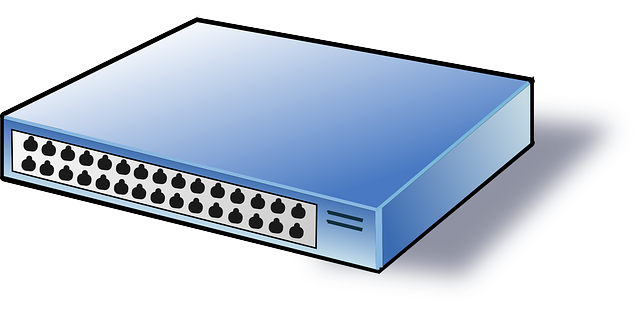
\includegraphics[scale=.3]{images/cartoon-switch}
    \end{figure}
\end{frame}


\begin{frame}{Introdução}
    \begin{itemize}
        \setlength{\itemsep}{.5cm}
        \item Sistemas de balanceamento de carga são baseados em políticas 
            de balanceamento.
        \item Os serviços modernos devem ser escaláveis para atender a 
            milhões ou milhares de clientes.
        \item Os serviços devem ser distribuídos em vários servidores. 
        \item O OpenFlow permite políticas que podem se adaptar à aplicação 
            ou serviço.
    \end{itemize} 
\end{frame}


\begin{frame}{Projeto de implementação}

    \begin{itemize}
        \setlength{\itemsep}{.5cm}
        \item A solução resume-se em um balanceador de carga TCP.
        \item Um IP lógico é atribuído ao serviço
        \item Políticas de balanceamento decidem quais servidores serão
            escalonados
    \end{itemize}

\end{frame}

\section{Proposta de solução}

\begin{frame}{Proposta de solução}

    \begin{figure}[h]
        \centering
        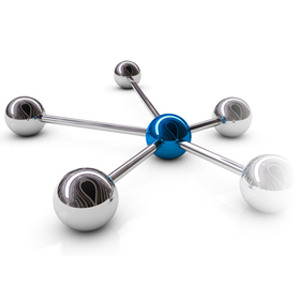
\includegraphics[scale=.8]{images/small-graph}
    \end{figure}
\end{frame}

\begin{frame}{Proposta de solução}
    
    \begin{itemize}
        \setlength{\itemsep}{.5cm}
        \item Uma abstração da rede em forma de um módulo em grafos 
        \item Esse grafo, em tempo real, é a base para computações na rede
        \item A solução objetiva simplificar a análise e o gerenciamento 
            em redes
    \end{itemize}

\end{frame}

\begin{frame}{Modelagem do grafo}

    \begin{itemize}
        \setlength{\itemsep}{.5cm}
        \item $G=(V, A)$, em que $V$ e $A$ são conjuntos finitos de vértices 
            e arestas, respectivamente.
        \item Cada vértice $v \in V$ é um computador ou \emph{switch}.
        \item Cada aresta $u \to v \in A$ é um enlace entre dois vértices.
        \item O peso das arestas $g(u, v)$ é quantidade de \emph{bytes} 
            trafegados na aresta entre os dois vértices.
    \end{itemize}
\end{frame}

\begin{frame}{Classes}

    \begin{columns}[T] % align columns
        \begin{column}{.33\textwidth}

            \begin{itemize}
                \setlength{\itemsep}{.5cm}
                \item{Graph}
                \item{GraphEntity}
                \item{Vertex}
                \item{Edges} 
                \item{GraphManager}
            \end{itemize}
        \end{column}%
        \hfill%
        \begin{column}{.67\textwidth}
            \begin{figure}[h]
                \centering
                
\includegraphics[scale=.4]{images/graph-interfaces}
            \end{figure}
        \end{column}%
    \end{columns}

\end{frame}

\begin{frame}{Interface de programação}

    \begin{columns}[T] % align columns
        \begin{column}{.33\textwidth}

            \begin{itemize}
                \setlength{\itemsep}{.5cm}
                \item \emph{get\_vertex(id)}
                \item \emph{get\_adjacents(id)}
                \item \emph{snapshot()}
                \item \emph{get\_mst()}
            \end{itemize}
        \end{column}%
        \hfill%
        \begin{column}{.67\textwidth}
            \begin{figure}[h]
                \centering
                
\includegraphics[scale=4]{images/gear}
            \end{figure}
        \end{column}%
    \end{columns}

\end{frame}

\begin{frame}{Integração entre módulos}

\begin{figure}[h!]
    \centering
    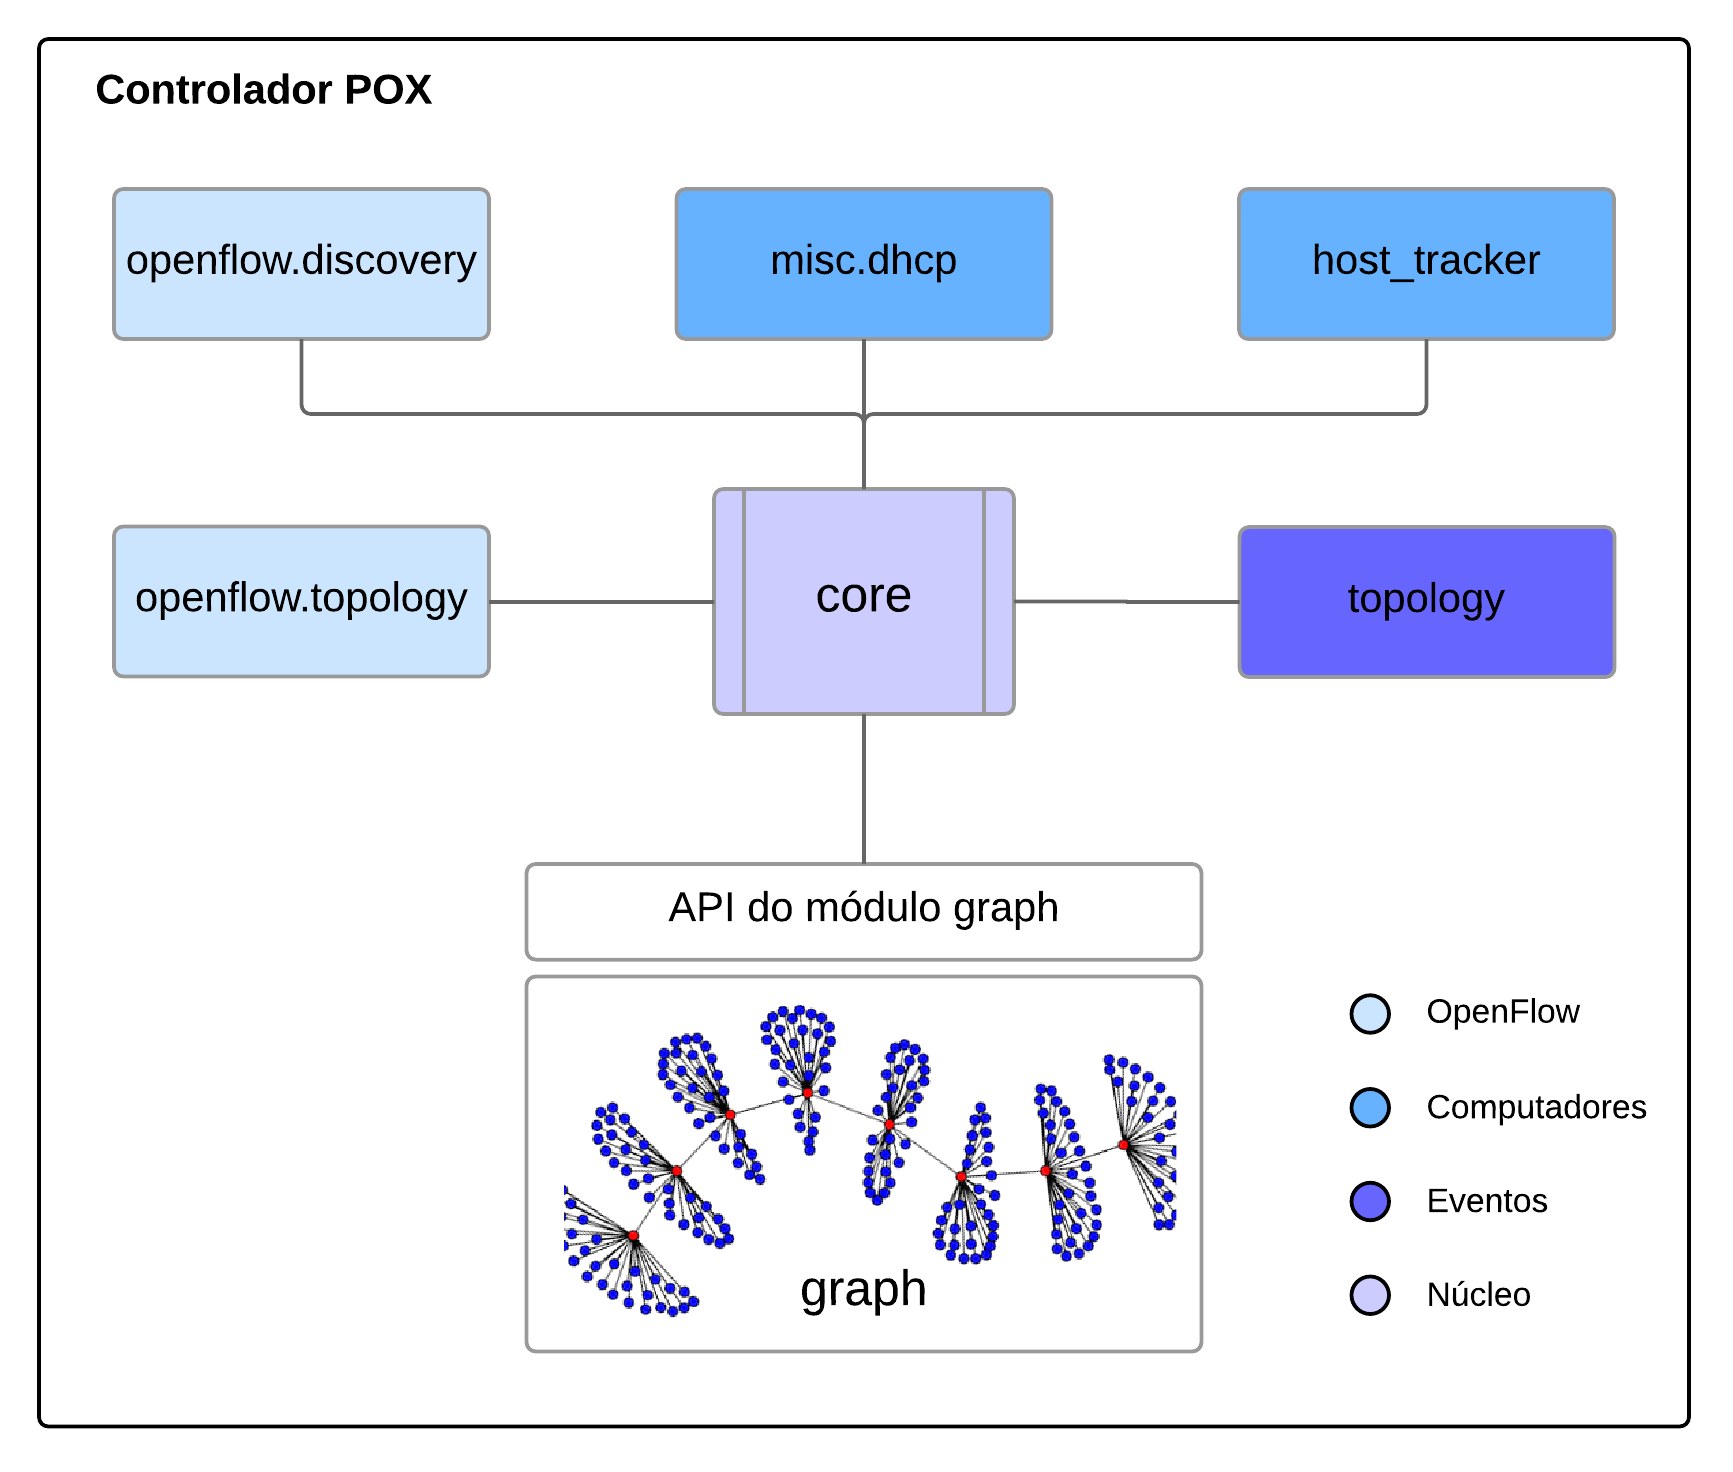
\includegraphics[scale=.55]{images/graph-module-integration}
\end{figure}

\end{frame}

\chapter{Experimentação e resultados}
\label{cap:experiments}

\section{Ambiente de simulação}

Uma simulação da rede nacional de pesquisa, a rede Ipê \citep{ipe2015network} 
foi criada em laboratório.
Um comutador (\emph{switch}) OpenFlow e quatro servidores foram utilizados 
para executar a simulação no laboratório WiNet \citep{winet22015lab}
no departamento de Ciência da Computação (DCC) da Universidade Federal 
de Minas Gerais (UFMG).

\subsection{A rede Ipê}
Operada pela Rede Nacioanal de Pesquisa (RNP), a rede Ipê é uma infraestrutura
de rede Internet dedicada à comunidade de pesquisa brasileira.
Inaugurada em 2005, foi a primeira rede óptica nacional acadêmica a entrar em
operação na América Latina.

A rede IPÊ implementa 27 Pontos de Presença (\emph{POPs}), um para cada unidade
da federação.
Em cada unidade existem diversos clientes que, para se comunicar com outras 
máquinas em outros Pontos de Presença, transmitem seus pacotes através do 
POP ao qual atuam como clientes.
Essas ramificações constituem mais de 800 instituições de ensino, saúde e 
pesquisa em todo o país, beneficiando mais de 3,5 milhões de usuários
\citep{ipe2015network}.

Através da rede RedCLARA \citep{redclara2015network}, a rede Ipê se conecta 
à 2,5 Gb/s com, atualmente, 15 países da América Latina e à 5 Gb/s com a rede
europeia Géant \citep{geant2015network}. 
Além disso, por meio de quatro conexões de
10 Gb/s, duas pelo Oceano Atlântico e duas pelo Oceano Pacífico, 
operadas em parceria com a ANSP, totalizando 40 Gb/s, a rede Ipê se conecta 
às redes acadêmicas norte-americanas, em especial, a  Internet2 
\citep{internet22015network}, a outras redes acadêmicas internacionais e à 
internet comercial mundial.

Os Pontos de presença estão interconectados conforme mostrado na figura 
\ref{fig:ipe-network-2015}.

\begin{figure}[!ht]
    \centering
    \label{fig:ipe-network-2015}
    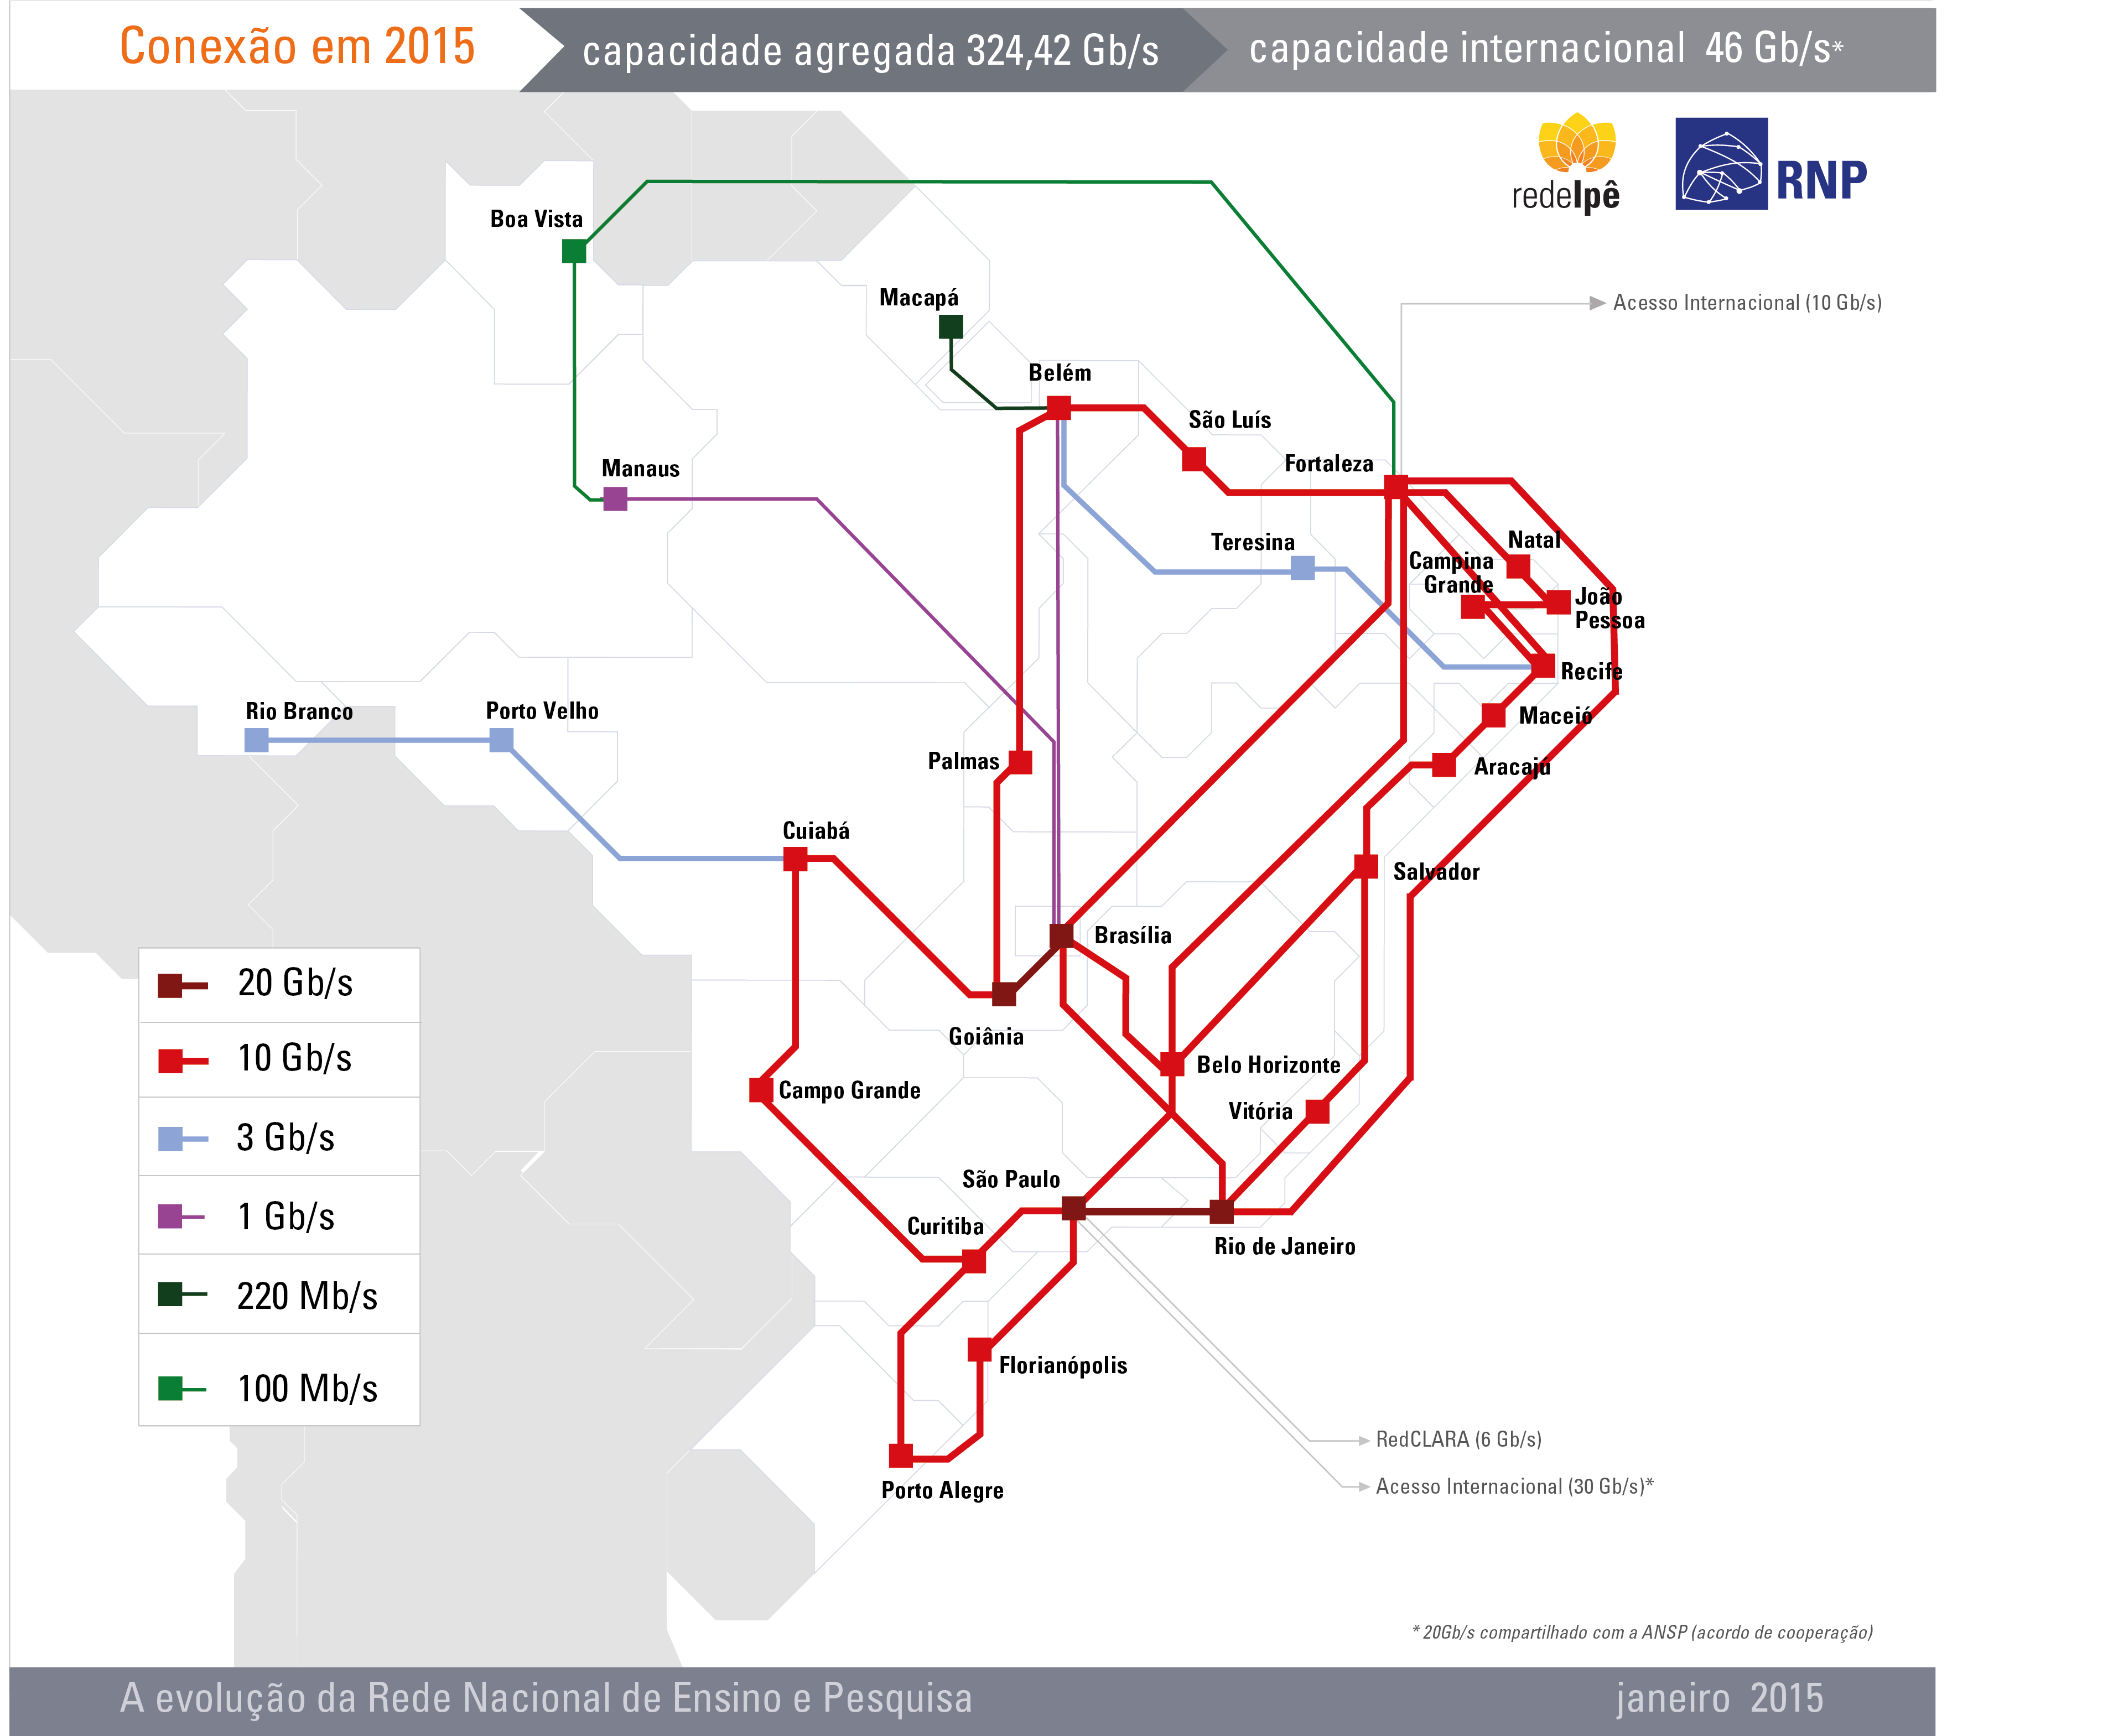
\includegraphics[width=\textwidth]{img/ipe-network-2015}
    \caption{Rede Nacional de Pesquisa IPÊ \protect\footnotemark}
    \vspace*{3in}
\end{figure}

\footnotetext{Imagem retirada de 
\url{http://www.rnp.br/servicos/conectividade/rede-ipe}}

\subsection{Arquitetura da simulação}

A ambiente de simulação é composto por um comutador HP com OpenFlow habilitado.
Quatro servidores são responsáveis por gerenciar máquinas virtuais que 
representam as unidades federativas e suas instituições clientes.

Conforme pode ser visto na figura \ref{fig:physical-vs-virtual-network}, a
rede física do esperimento é separada da rede virtual.
O quinto computador é o controlador da rede. 
Para o experimento, existem duas redes. 
Uma rede de administração, com acesso aos servidores e a uma instância do 
controlador, na porta 6633.
A segunda rede é a rede virtual à qual todos os POPs simulados estão 
conectados. 
Para implementar essas duas redes, cada servidor e o controlador possuem duas
interfaces de rede que isolam seus funcionamentos.
Assim, a rede física/administrativa e a rede virtual/Ipê estão separadas
em nosso experimento.


\begin{figure}[!h]
    \centering
    \label{fig:physical-vs-virtual-network}
    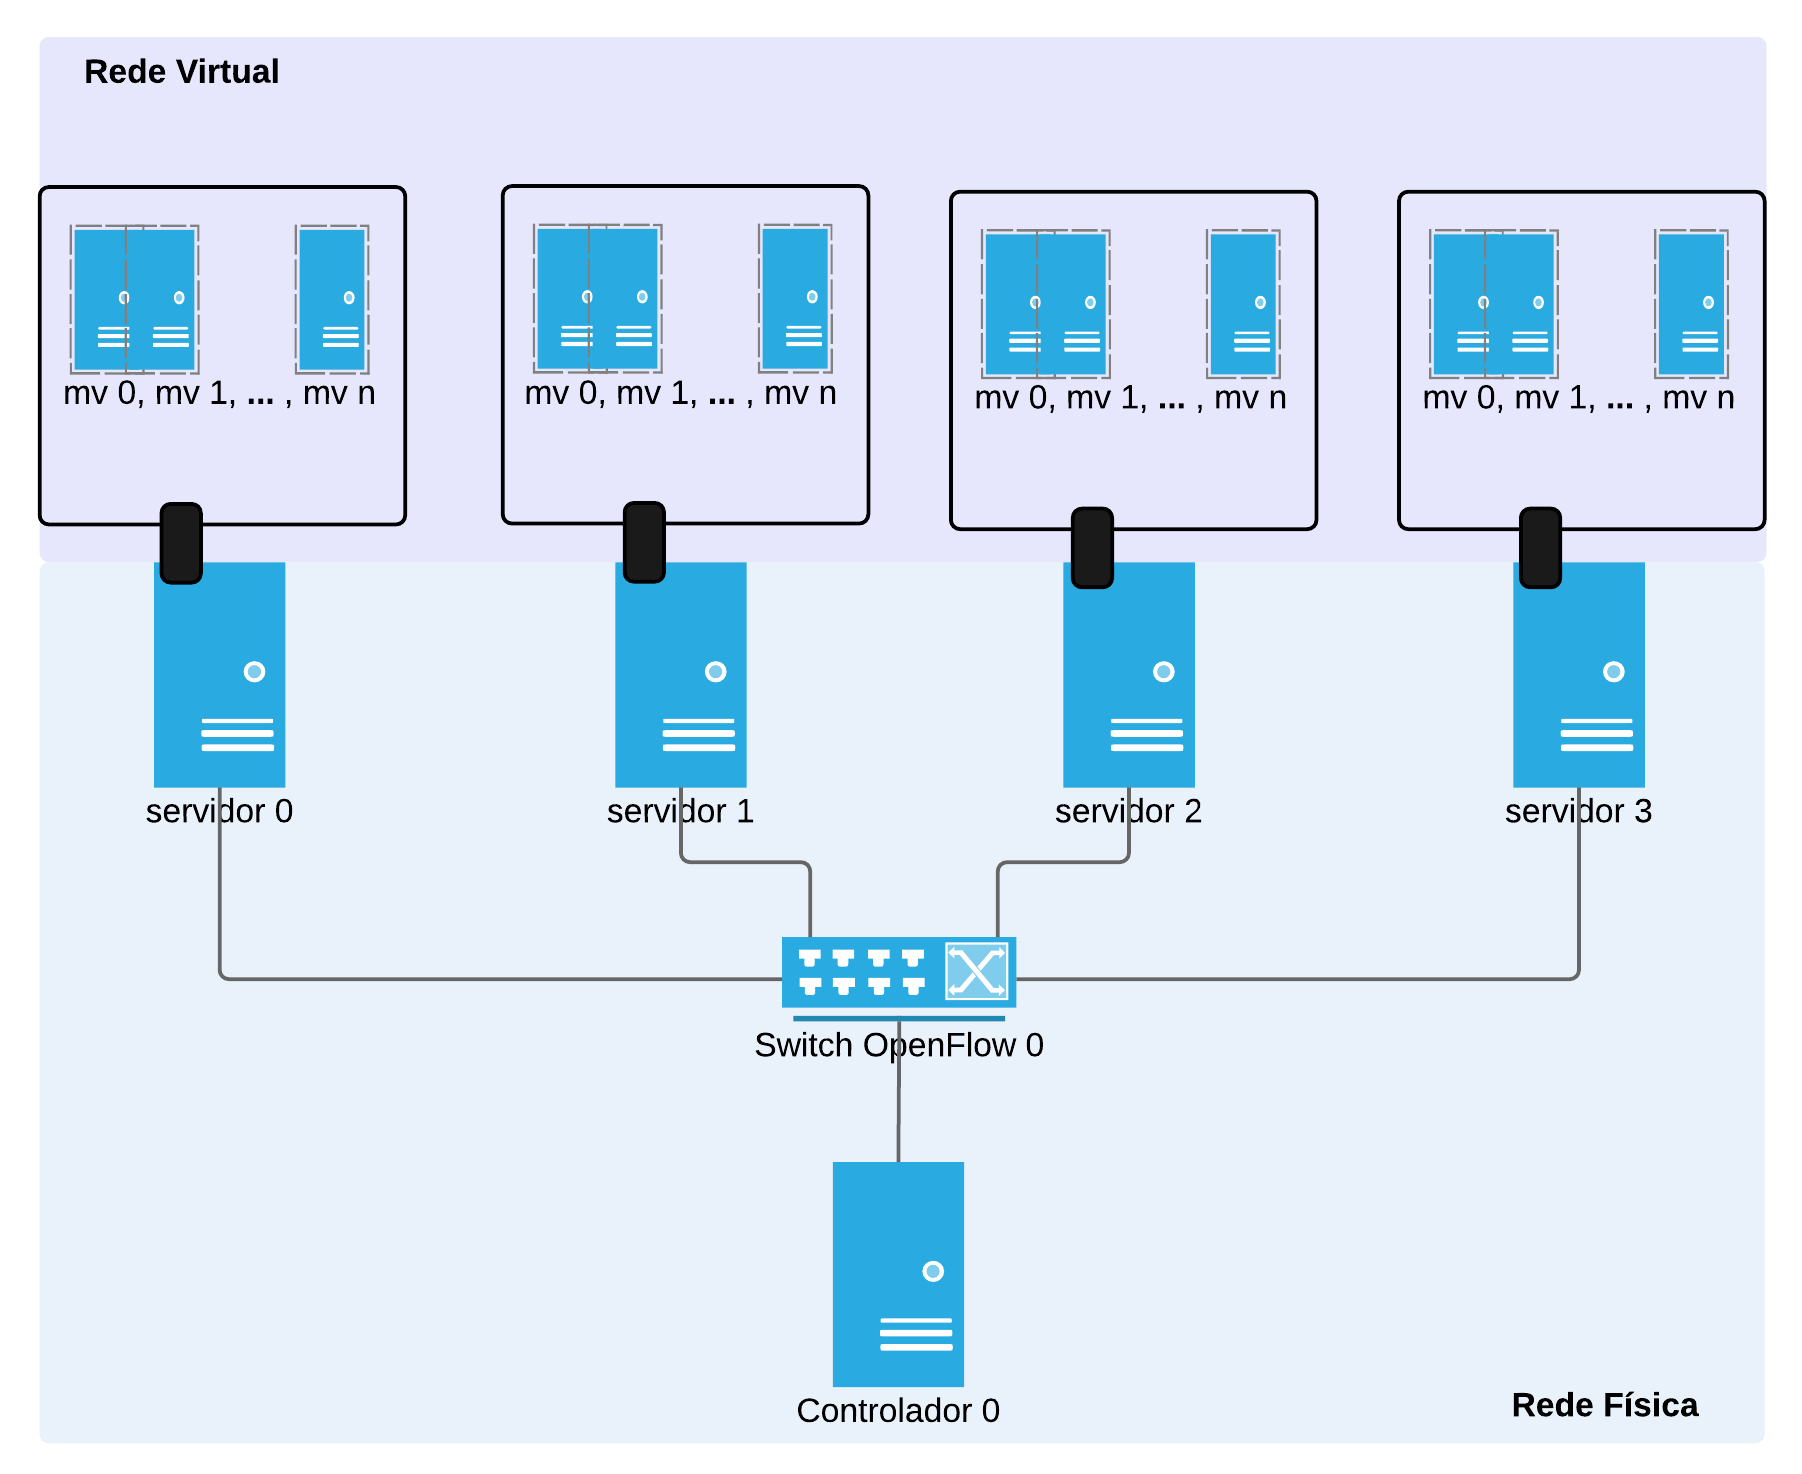
\includegraphics[width=\textwidth]{img/physical-vs-virtual-network-pt}
    \caption{Arquitetura do ambiente de simulação}
\end{figure}

Para o ambiente virtualizado, o controlador está associado a porta 6653.
Cada POP é um comutador (\emph{switch}) OpenFlow simulado via OpenVSwitch
\citep{openvswitch2015switch}.
As instituições clientes de cada POP são simuladas através do \emph{Mininet} 
\citep{lantz2010network}.
O número de instituições clientes foi coletado do sítio de cada Ponto de 
Presença.

Cada máquina virtual representa um POP.
Cada POP possui uma subrede à qual uma instância do \emph{Mininet} simula 
seus clientes. 
Essa subrede está conectada através de um \emph{switch} virtual 
\emph{OpenVSwitch} que é controlado pelo controlador da rede virtualizada.
Assim, para cada POP, temos as decisões e atualizações da tabela de fluxos
feita pelo controlador.
Toda comunicação de saída das subredes utilizando \emph{mininet} passam pelo 
\emph{OpenVSwitch} que funciona em modo \emph{bridge} (ponte) com a interface
de rede virtual conforme pode ser visto na figura
\ref{fig:mininet-vm-architecture}.


\begin{figure}[h!]
    \centering
    \label{fig:mininet-vm-architecture}
    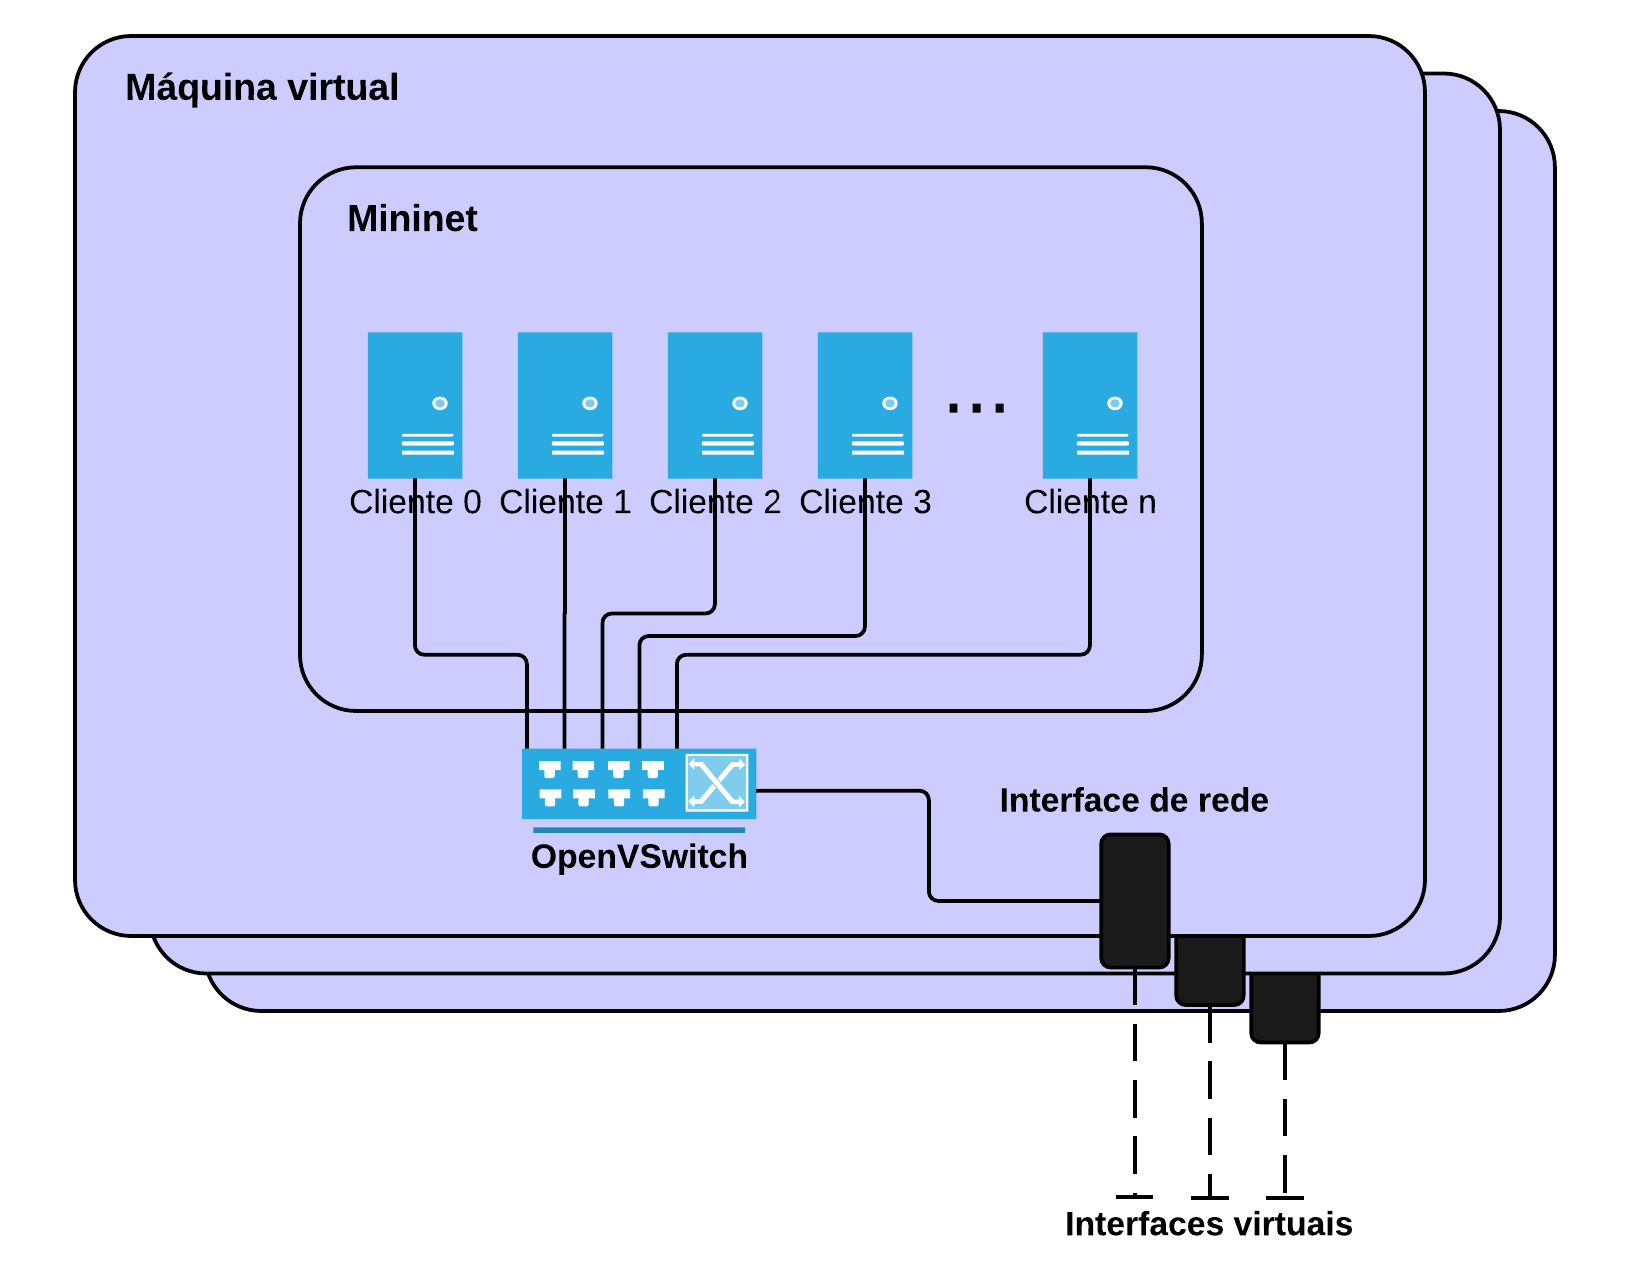
\includegraphics{img/mininet-vm-architecture}
    \caption{Arquitetura de cada máquina virtual}
\end{figure}


A tabela \ref{tbl:testbed-ipe-net} apresenta as subredes de cada unidade
federativa (POP), qual servidor físico gerencia a máquina virtual referente
ao POP e o número de clientes a ele associado.

\begin{table}[h]
    \label{tbl:testbed-ipe-net}
    \centering
    \resizebox*{!}{\dimexpr\textheight- 25px}{
    \resizebox{\linewidth}{!}{
    \begin{tabular}{llllll}
        \rowcolor[HTML]{000000} 
        \multicolumn{6}{c}{\cellcolor[HTML]{000000}{\color[HTML]{C0C0C0} 
            \textbf{Associação de Servidores à simulação da rede IPÊ}}} \\
        \rowcolor[HTML]{000000} 
        {\color[HTML]{9B9B9B} \textbf{UF}} & {\color[HTML]{9B9B9B} 
            \textbf{N clientes}} & {\color[HTML]{9B9B9B} 
            \textbf{Sub-rede local}} & {\color[HTML]{9B9B9B} 
            \textbf{Servidor}} & {\color[HTML]{9B9B9B} \textbf{IP local}} & 
            {\color[HTML]{9B9B9B} \textbf{IP Gateway}} \\
        AC &  10 &  10.10.1.0 &   Shiva  &  10.10.42.51 & \\ 
        AL  & 13 &  10.10.2.0  &  Shiva  &  10.10.42.52 & \\ 
        AM  & 20 &  10.10.3.0 &   Shiva  &  10.10.42.53 & \\
        AP  & 7  &  10.10.4.0 &   Shiva  &  10.10.42.54 & 10.10.42.50 \\
        BA  & 25 &  10.10.5.0 &   Shiva  &  10.10.42.55 & \\
        CE  & 50  & 10.10.6.0  &  Shiva  &  10.10.42.56 & \\
        DF  & 16 &  10.10.7.0  &  Shiva  &  10.10.42.57 & \\ \hline
        ES  & 26  & 10.10.8.0  &  Eden  &   10.10.42.101 & \\
        GO  & 26  & 10.10.9.0  &  Eden  &   10.10.42.102  & \\  
        MA  & 7  &  10.10.10.0 &  Eden  &   10.10.42.103  & \\  
        MG  & 32  & 10.10.11.0  & Eden  &   10.10.42.104  & 10.10.42.100 \\  
        MS  & 10  & 10.10.12.0  & Eden  &   10.10.42.105  & \\  
        MT  & 8   & 10.10.13.0  & Eden  &   10.10.42.106  & \\  
        PA  & 13  & 10.10.14.0  & Eden  &   10.10.42.107  & \\ \hline
        PB  & 14  & 10.10.15.0  & Diablos & 10.10.42.151  & \\
        PE  & 41  & 10.10.16.0  & Diablos & 10.10.42.152  & \\  
        PI &  25 &  10.10.17.0 &  Diablos & 10.10.42.153  & \\  
        PR &  71 &  10.10.18.0 &  Diablos & 10.10.42.154  & 10.10.42.150 \\
        RJ &  27 &  10.10.19.0 &  Diablos & 10.10.42.155  & \\  
        RN &  11 &  10.10.20.0 &  Diablos & 10.10.42.156  & \\  
        RO &  10 &  10.10.21.0 &  Diablos & 10.10.42.157  & \\ \hline
        RR  & 7  &  10.10.22.0 &  Leviathan &   10.10.42.201 & \\
        RS &  10 &  10.10.23.0 &  Leviathan &   10.10.42.202  & \\  
        SC &  47 &  10.10.24.0 &  Leviathan &   10.10.42.203 & 10.10.42.200 \\   
        SE &  13 &  10.10.25.0 &  Leviathan &   10.10.42.204 & \\   
        SP &  25 &  10.10.26.0 &  Leviathan &   10.10.42.205  & \\  
        TO &  11 &  10.10.27.0 &  Leviathan &   10.10.42.206 & \\   
    \end{tabular}
    }}
\end{table}



\section{Detecção de entidades}

Ao ser carregado, o módulo \emph{graph} inicia o grafo da rede vazio.
Os \emph{switches} são os primeiros a serem identificados. 
Como o controlador está ligado diretamente a eles pela interface
\emph{OpenFlow}, um evento de \emph{ConnectionUp} é disparado 
pelo núcleo do controlador.
Esse evento dispara o evento \emph{SwitchJoin} através do módulo 
\emph{topology} que faz com que o grafo adicione vértices.

\begin{figure}[h!]
    \centering
    \begin{lstlisting}[ tabsize=4,  
                        language=bash,
                        basicstyle=\ttfamily\footnotesize,
                        aboveskip={1.5\baselineskip},
                        columns=fixed,
                        showstringspaces=false,
                        extendedchars=true,
                        breaklines=true,
                        frame=single,
                        numbers=left,
                        showtabs=false,
                        showspaces=false,
                        showstringspaces=false,
                        identifierstyle=\ttfamily,
                        ]
INFO:topology.graph:SwitchJoin id: 2
INFO:topology.graph:SwitchJoin id: 1
INFO:topology.graph:1, 2
DEBUG:openflow.discovery:Dropping LLDP packet 275
INFO:topology.graph:LinkEvent fired
INFO:host_tracker:Learned 1 1 7e:e6:9b:89:39:2e got IP 10.0.0.1
INFO:topology.graph:HostJoin id: 7e:e6:9b:89:39:2e
INFO:host_tracker:Learned 2 1 62:77:44:24:13:49 got IP 10.0.0.2
INFO:topology.graph:HostJoin id: 62:77:44:24:13:49
        \end{lstlisting}
    \caption{Detecção de entidades}
    \label{fig:detection}
\end{figure}

Nas duas primeiras linhas do \emph{log} mostrado na figura
\ref{fig:detection}, o módulo \emph{graph} foi notificado
da descoberta de dois \emph{switches} na rede.
Na linha 5, nota-se a descoberta de um enlace (\emph{link}) entre dois
comutadores (\emph{switches}).
O módulo \emph{openflow.discovery}, através do protocolo LLDP identificou 
o link entre \emph{switches}.
O grafo foi notificado e estabeleceu uma aresta entre os 
vértices (\emph{switches}).

As linhas 7 e 9 mostram a descoberta de dois hosts.
Esses hosts foram descobertos pelo módulo \emph{host\_tracker} via 
escuta dos eventos de DHCP.
É importante ressaltar que a descoberta de \emph{hosts} também ocorre 
independente do DHCP.
Um novo pacote que passa por um \emph{switch} e não possui regra
instalada na tabela de fluxos é encaminhado ao controlador que 
dispara um evento de \emph{PacketIn}. 
Para tal, o \emph{host\_tracker} se encarrega de escutar esse evento 
e notificar o grafo através do evento \emph{HostJoin} disparado pelo módulo
\emph{topology} ao criar um novo \emph{Host}.
O grafo, ao ser notificado, cria vértices para esses \emph{hosts} associando 
uma aresta entre eles e o \emph{switch} ao qual eles estão conectados.
Dessa forma as entidades da rede são identificadas e computadas no grafo.


\section{Remoção de entidades}

\subsection{Remoção de computadores}

Diversos computadores foram desligados de maneira aleatória.
O \emph{host\_tracker}, após um tempo fixo (\emph{timerInterval}) 
verifica via ARPPing se os \emph{hosts} conhecidos estão ativos.
Para esse cenário da remoção de um computador (\emph{host}), 
o \emph{host\_tracker} identifica a inatividade do \emph{host} e remove o 
\emph{Host}.
O evento de \emph{HostLeave} é disparado pelo \emph{topology}, 
atualizando assim o grafo.

Nesse cenário de experimento, cinco computadores de cada subrede foi desligado.
Para cada computador foi coletado o tempo em que ele foi desligado.
Quando o controlador, através do \emph{host\_tracker}, identifica a saída 
desse computador o tempo é novamente coletado.
Assim, para cada computador desligado, foi computado o tempo decorrido até 
que o controlador o removesse do grafo da rede.

\begin{figure}[h!]
    \centering
    \label{fig:hosts-leave-time}
    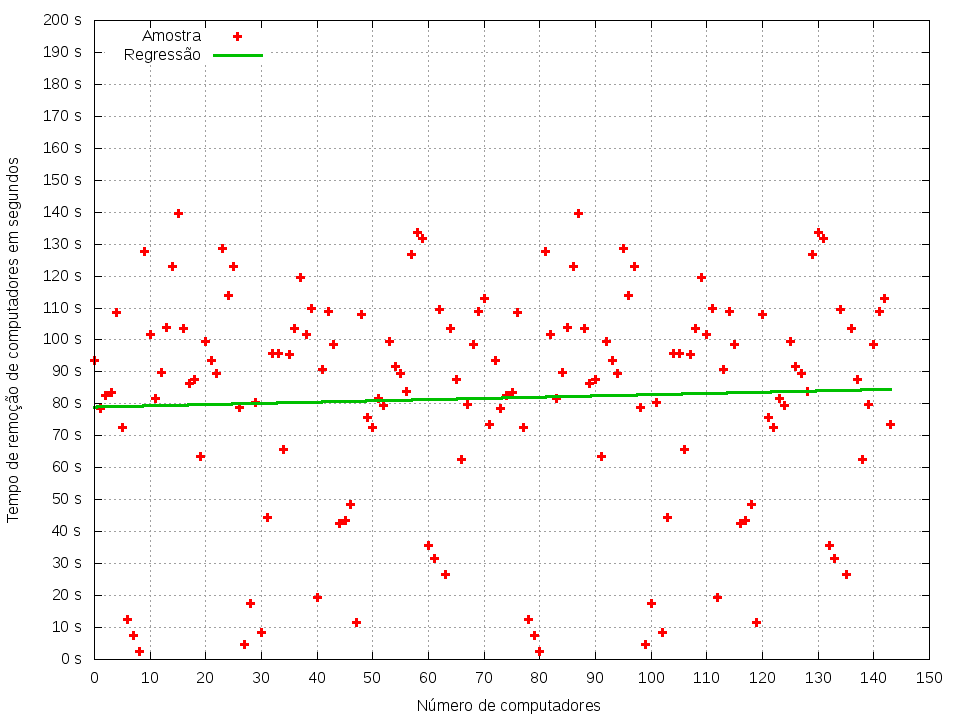
\includegraphics[width=\linewidth]{img/hosts-leave-time}
    \caption{Tempo decorrido entre o desligamento de um computador e a 
    remoção do mesmo no grafo}
\end{figure}

Os resultados da amostra coletada pode ser visto na figura
\ref{fig:hosts-leave-time}.
Em média, o tempo de remoção de um computador do grafo demorou 80 segundos.
A sondagem foi configurada para ser executada com uma periodicidade de 60 
segundos. 
A regressão linear computada mostra que esse valor médio é praticamente 
constante ao longo dos valores amostrados.

Computadores cuja remoção ocorreram em um intervalo de tempo muito reduzido
tiveram seu tempo de sondagem expirado muito próximos ao momento em que 
o \emph{host\_tracker} executava sua sondagem. 

\subsection{Remoção de comutadores}

Para o caso de comutadores (\emph{switch}), foram desligados os 
\emph{switches} e medido o tempo de atualização do grafo.
O controlador está ligado diretamente aos \emph{switch}. 
Em função disso os comutadores são removidos mais rapidamente do grafo.
A figura \ref{fig:switch-leave-time} apresenta os resultados da 
computação da amostra de \emph{switches} removidos.
Assim, ao ser desligado, o \emph{core} do POX dispara um evento 
de \emph{SwitchLeave} ao qual o módulo \emph{graph} está inscrito. 
Logo, o grafo é atualizado removendo o vértice do \emph{switch}.

\begin{figure}[h!]
    \centering
    \label{fig:switch-leave-time}
    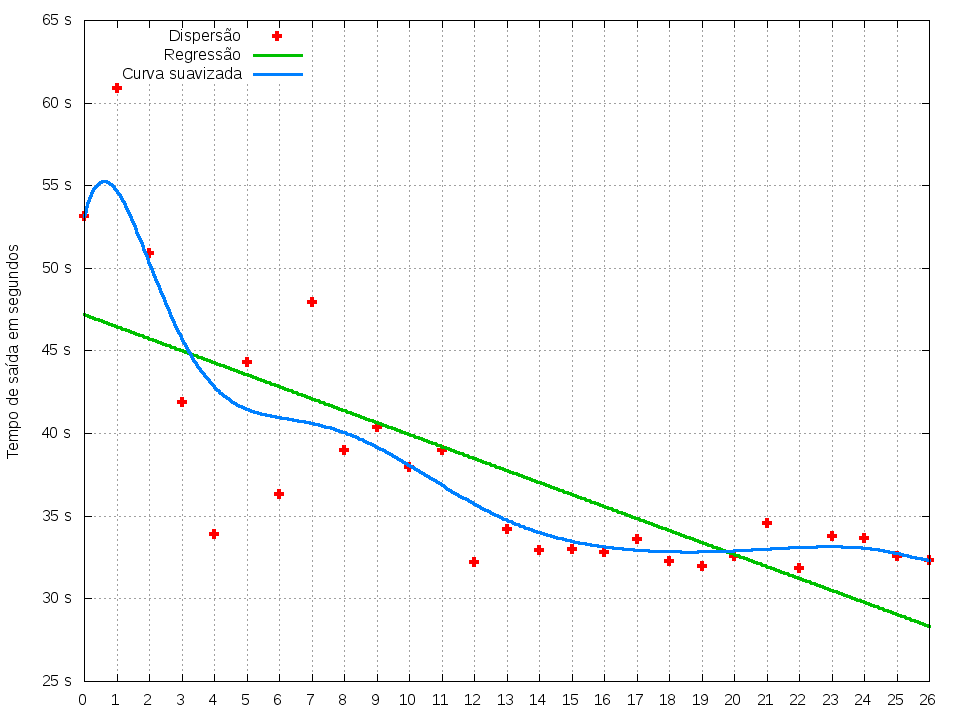
\includegraphics[width=\linewidth]{img/switch-leave-time}
    \caption{Tempo decorrido entre o desligamento de um comutador 
    (\emph{switch}) e a remoção do mesmo no grafo}
\end{figure}

Uma curva suavizada da interpolação dos pontos mostra que apesar dos valores
de tempo mais elevados nos primeiros valores da amostra, ao final esses valores
são praticamente constantes, em um valor de 30 a 35 segundos para cada 
remoção.

Após algum tempo o \emph{host\_tracker} identifica se os computadores 
associados ao \emph{switch} removido estão ativos por outra rota. 
Caso negativo, os computadores são removidos do grafo.
Considerando o experimento da remoção dos comutadores (\emph{switches}),
foi computado o tempo decorrido entre a remoção do \emph{switch} e a 
remoção dos computadores na rede interna ao \emph{switch}. 

\begin{figure}[h!]
    \centering
    \label{fig:hosts-behind-switch-time}
    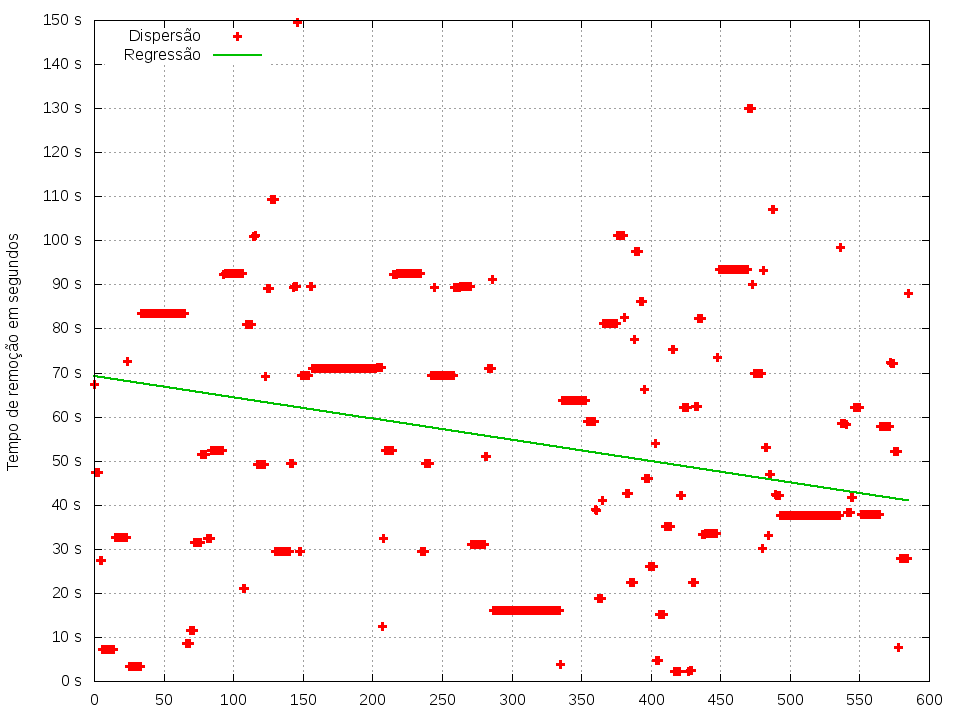
\includegraphics[width=\linewidth]{img/hosts-behind-switch-time}
    \caption{Tempo decorrido entre a remoção dos comutadores 
    (\emph{switches}) e a remoção dos computadores na rede interna ao 
    \emph(switch)}
\end{figure}

A figura \ref{fig:hosts-behind-switch-time} mostra o resultado do experimento
para o tempo de remoção de computadores em função da remoção do 
\emph{switch}.
Os resultados mostram uma média que varia entre 40 e 70 segundos para a 
remoção dos computadores.
No geral nota-se que computadores de uma mesma subrede foram removidos em 
instantes próximos.
Isso pode ser notado pelos pequenos grupos de pontos muito próximos na 
figura.

\section{Visualização em tempo real}

Uma imagem representando o grafo da rede é gerada pelo módulo \emph{graph}.
Essa imagem consiste na representação da topologia da rede no instante 
em que foi gerada. 
Periodicamente uma nova imagem é criada.
Um exemplo de grafo é apresentado na figura \ref{fig:full-graph}.
Essa figura representa uma rede simulada, dentro do ambiente do 
\emph{Mininet}, com 8 comutadores (\emph{switches}), cada um com 30 
computadores (\emph{hosts}) conectados.

Essa topologia totaliza 248 entidades na rede.
Na figura, os vértices vermelhos representam os comutadores.
Os vértices azuis, os computadores.
Cada aresta é um enlace entre dois vértices.

Atualizações na topologia como, remover e adicionar entidades na rede, foram
executados.
A visualização da rede atualiza junto com as alterações no grafo.

\begin{figure}[h!]
    \centering
    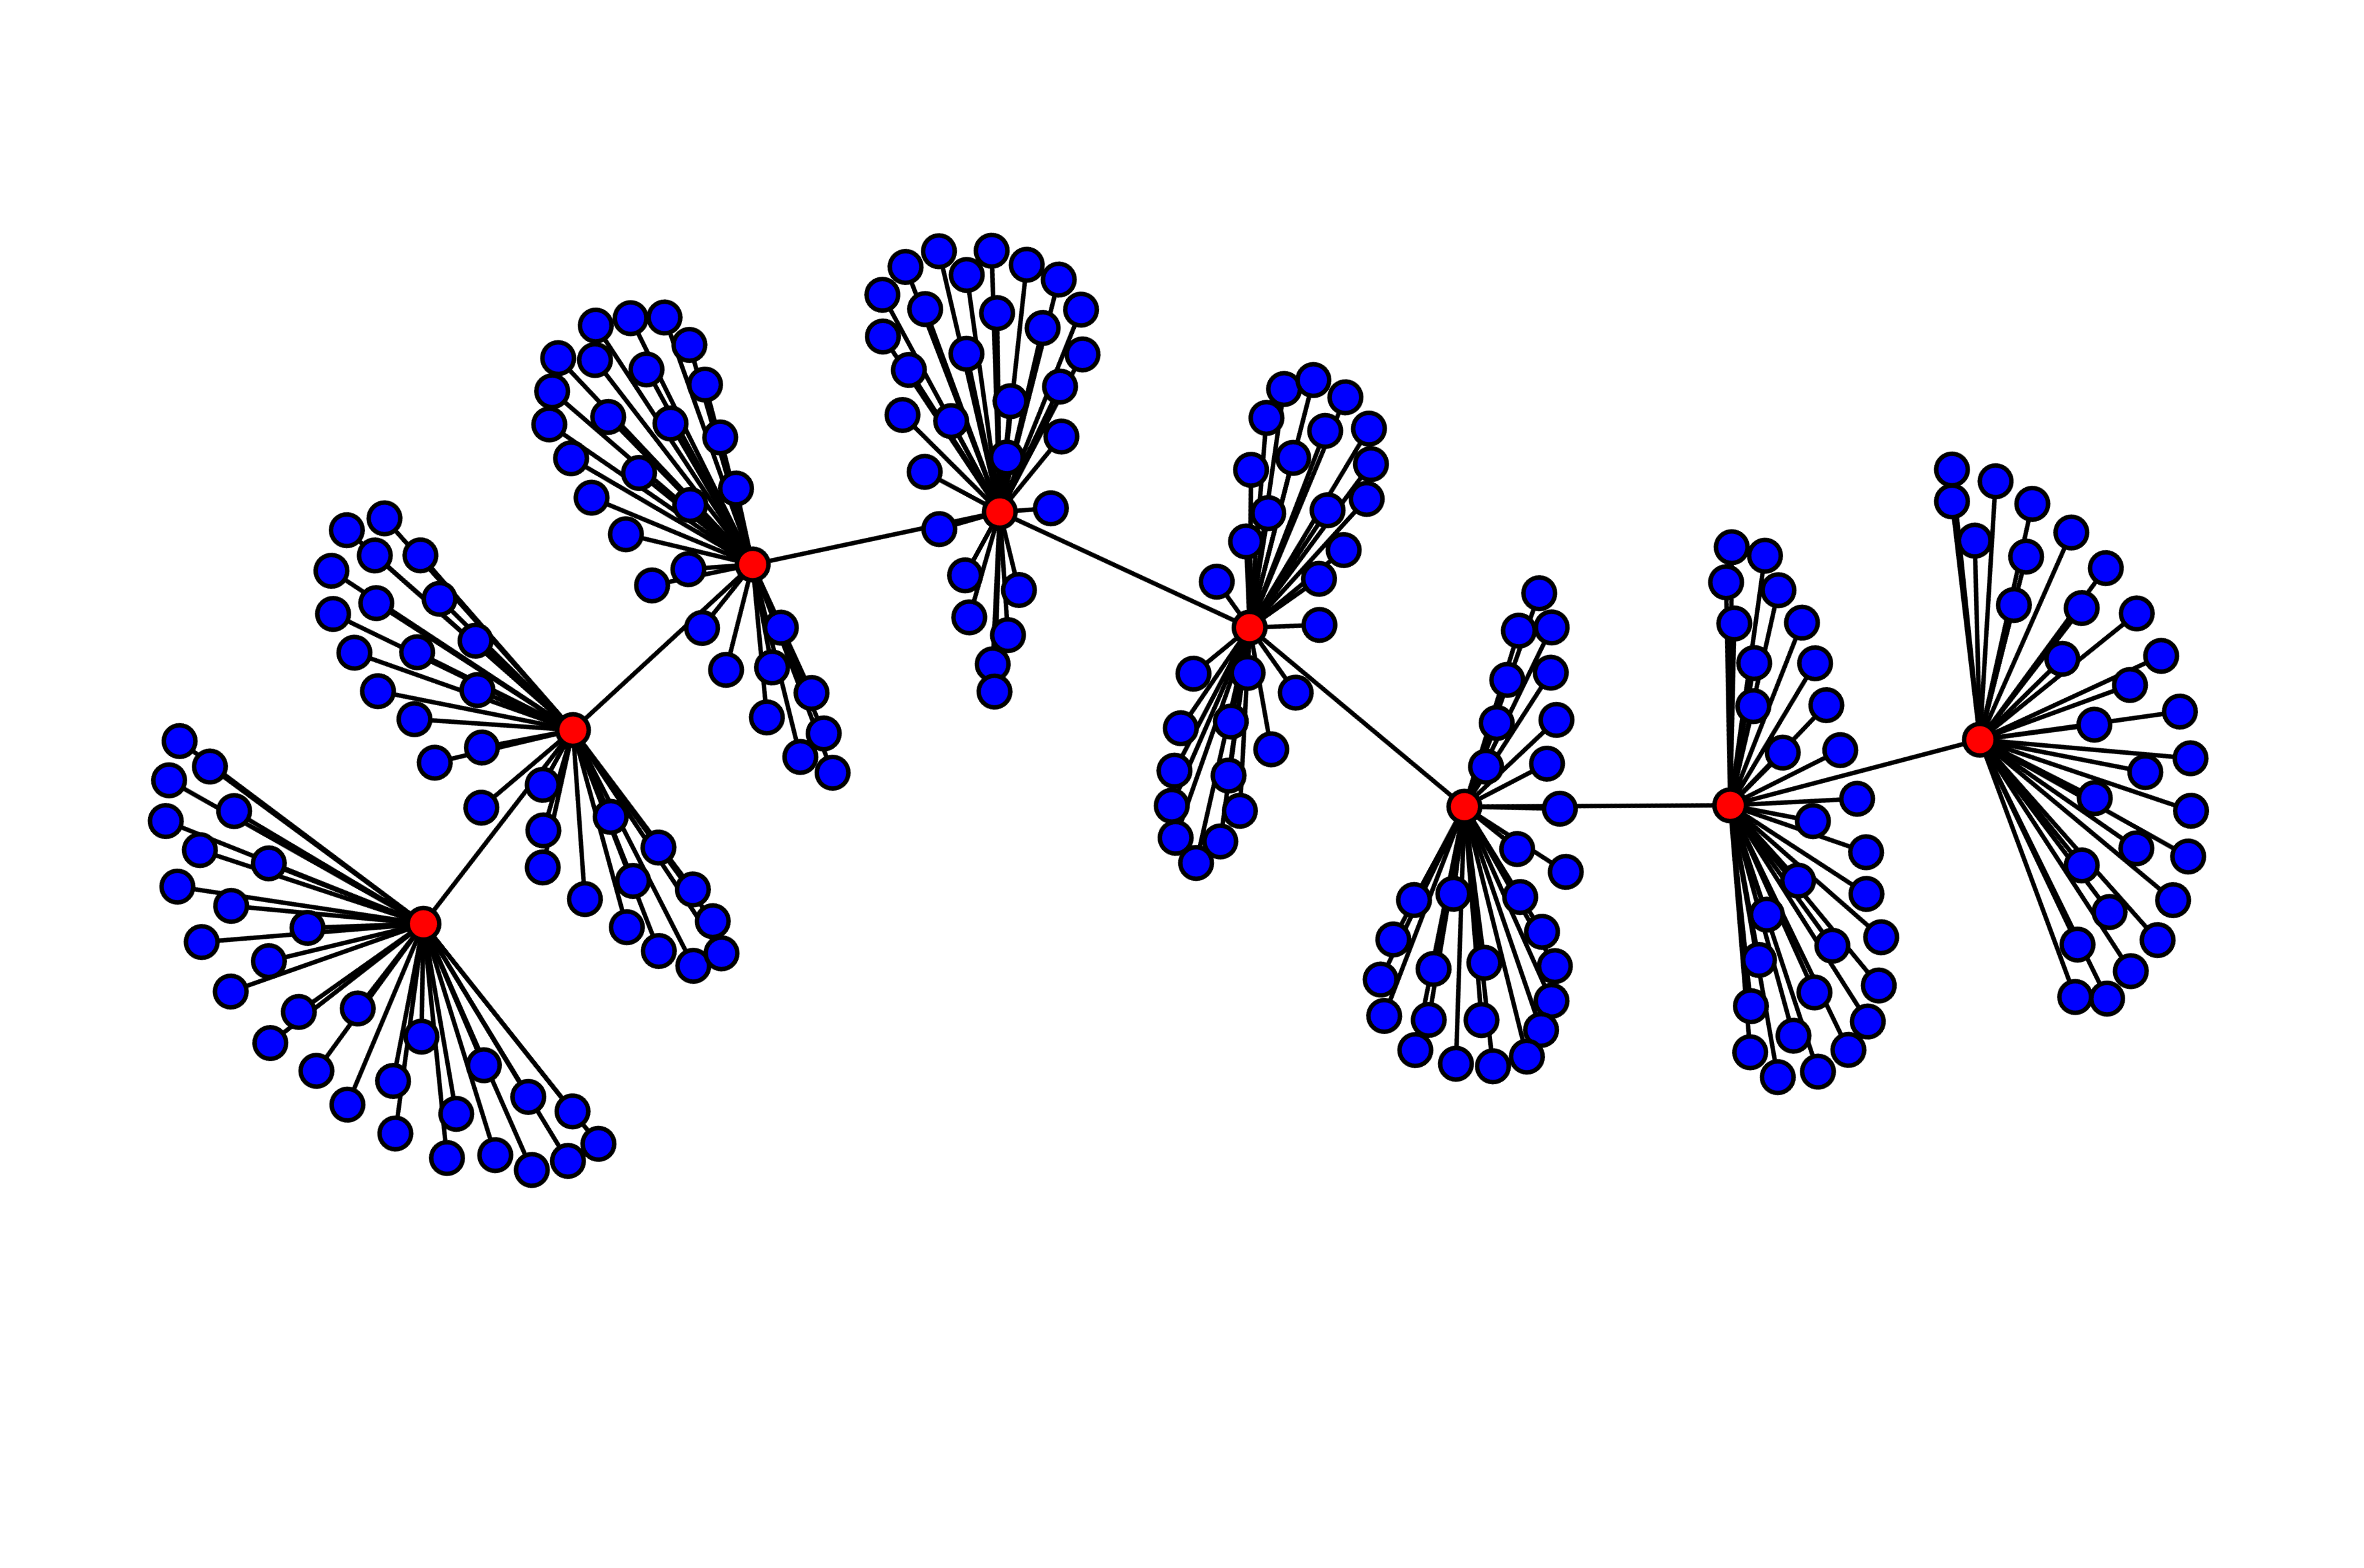
\includegraphics[width=\textwidth]{img/full-graph}
    \caption{Grafo representando uma rede com 248 entidades}
    \label{fig:full-graph}
\end{figure}
\break
Um experimento foi executado na rede Ipê para mostrar as alterações na 
representação do grafo.

No instante inicial, o controlador é iniciado.
Cada comutador estabelece uma conexão segura com o controlador.
Nesse momento, todos os vértices comutadores são adicionados ao grafo.
No segundo instante, para apenas uma subrede, representando uma unidade 
federativa dentro da rede Ipê, foi simulado tráfego entre seus computadores.
Para cada computador, uma sondagem de todos os outros computadores dessa
subrede foi feita através do utilitário \emph{ping}.
Assim, todas as máquinas dessa subrede foram identificadas pelo controlador
e adicionadas ao grafo representando a rede.
No terceiro instante, outra subrede foi escolhida e a mesma simulação de 
tráfego foi executada.
O mesmo procedimento foi repetido até que todas as 27 subredes da rede Ipê
fossem computadas pelo grafo.

A figura \ref{fig:full-graph-ipe} apresenta a execução desse experimento 
cronologicamente.
Cada número representa a quantidade de redes computadas pelo grafo no instante
da execução do experimento. 
Uma rede com 563 computadores e 27 comutadores (\emph{switches}) é mostrada
na imagem Final da figura \ref{fig:full-graph-ipe} representando toda a rede
Ipê.
No total o grafo computou 590 vértices.

\begin{figure}[htb!]
    \centering
    \label{fig:full-graph-ipe}
    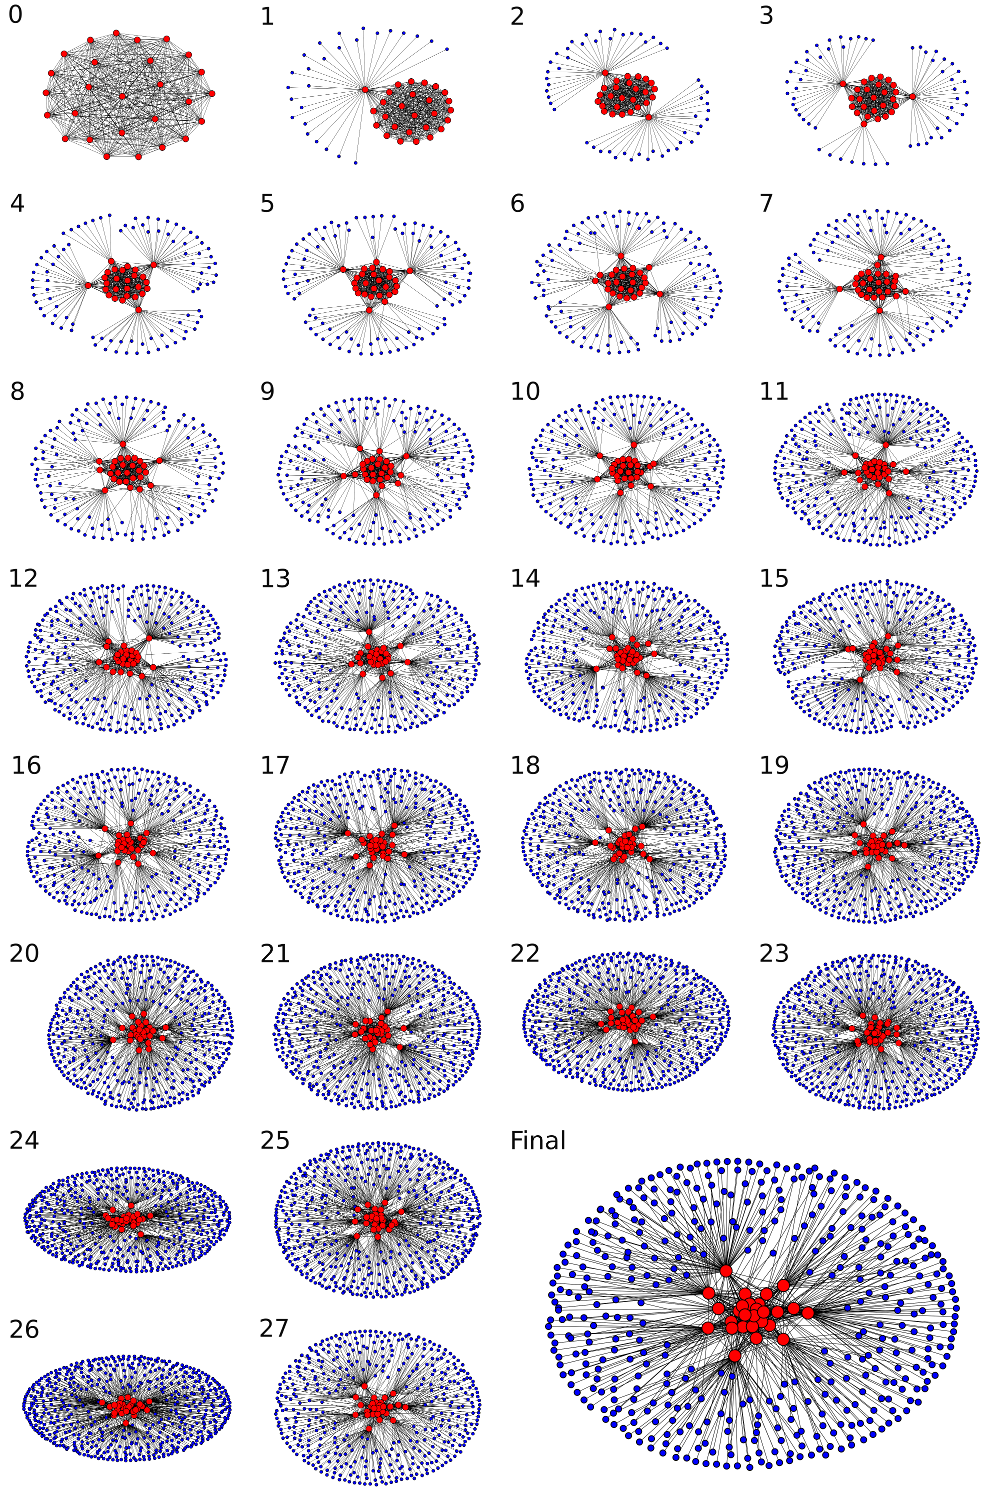
\includegraphics[scale=0.395]{img/full-graph-ipe}
    \caption{Representação da rede Ipê à medida que os computadores de cada
    subrede são identificados}
\end{figure}


\section{Identificação de tráfego}

Para computar o tráfego (TCP) em uma rede simples foi executado o programa 
\emph{iperf} como servidor no \emph{host} 'Host 0a'.
A topologia dessa rede é composta por dois comutadores interligados.
Cada comutador possui três computadores em cada subrede.
O \emph{host} 'Host 1e' conecta-se como cliente. 

Conformo pode ser notado na figura \ref{fig:iperf}, o tráfego 
em bytes na arestas desses \emph{hosts} é superior ao demais \emph{hosts}.
No momento em que foram lidos os contadores \emph{OpenFlow} e computados
os pesos das arestas, obteve-se um tráfego de 55894 bytes através do caminho
entre os dois \emph{hosts} citados.
Os valores apresentados para os demais \emph{hosts} (41 bytes) são referentes
ao tráfego ARP PING disseminado pelo módulo \emph{host\_tracker}

\begin{figure}[h!]
    \centering
    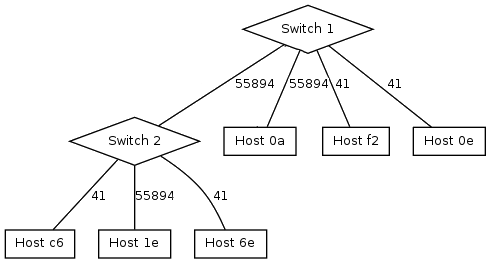
\includegraphics[scale=0.8]{img/graph-iperf}
    \caption{Tráfego TCP (em bytes) entre os hosts ’Host 1e’ e ’Host 0a’}
    \label{fig:iperf}
\end{figure}

\section{Avaliação do Controlador}

O consumo da unidade central de processamento (CPU) no processo do controlador,
no sistema operacional, assim como a utilização de memória e taxa de escrita 
em disco foram medidos através da biblioteca utilitária \emph{sysstat} 
\citep{sebastien2015sysstat}.

Um experimento variando o número de computadores na rede permitiu coletar 
as métricas citadas acima.
Coletou-se durante 30 segundos a utilização da CPU do processo do controlador,
do sistema operacional, a utilização de memória e a taxa de escrita em disco
em cada interação da execuçao do experimento.
A cada iteração do experimento, 50 novos computadores foram adicionados a rede.
Ou seja, o experimento começou com 50 computadores e terminou com 550.

\subsection{Consumo de processador no processo do controlador}


Conforme pode ser visto na figura \ref{fig:usr-cpu-growth}, considerando a 
variação das medições feitas no experimento, o crescimento da curva de 
utilização de CPU mostra-se logarítmica.
Apesar desse comportamento para o processo do controlador, nota-se que o 
consumo, analisando todo o sistema, é linear.
Esses resultados são apresentados na próxima seção. 
O comportamento logarítmo mostra que, apesar do aumento do número de
computadores na rede, o processo do controlador não gerou exaustão na CPU 
alocada para o processo ao longo do experimento.
À medida que a rede cresce, a utilização da CPU escalonada ao processo do 
controlador, cresce na mesma proporção.

\begin{figure}[htb!]
    \centering
    \label{fig:usr-cpu-growth}
    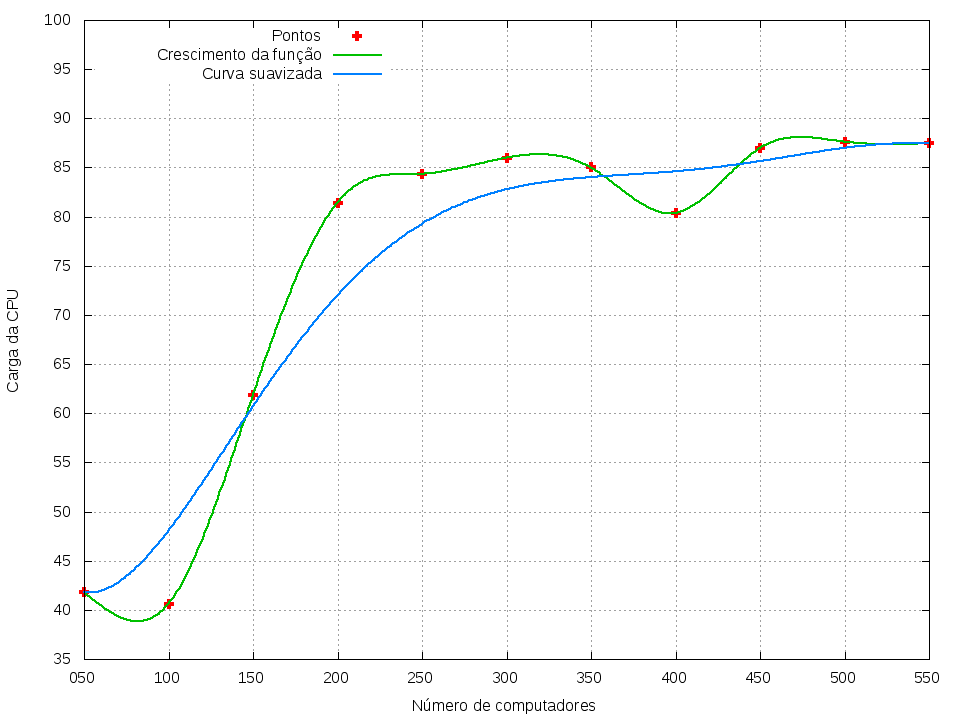
\includegraphics[width=\linewidth]{img/usr-cpu-growth.png}
    \caption{Variação do consumo médio de CPU no processo do controlador à 
    medida que a rede cresce}
\end{figure}

Uma regressão linear foi computada em cima da amostra coletada da utilização 
de CPU pelo processo do controlador.
A figura \ref{fig:scatter-usr-cpu} apresenta os resultados dessa computação.
É possível notar o crescimento da utilização de CPU à medida que a rede cresce.
A dispersão dos valores no início da amostragem estão mais próximos de 0. 
Ou seja, a rede com poucos computadores demandou baixo processamento. 
Já nos instantes finais, há mais pontos amostrados próximos a 100\% da 
utilização de CPU, o que mostra o estress do processador com uma rede maior.

\begin{figure}[!htb]
    \centering
    \label{fig:scatter-usr-cpu}
    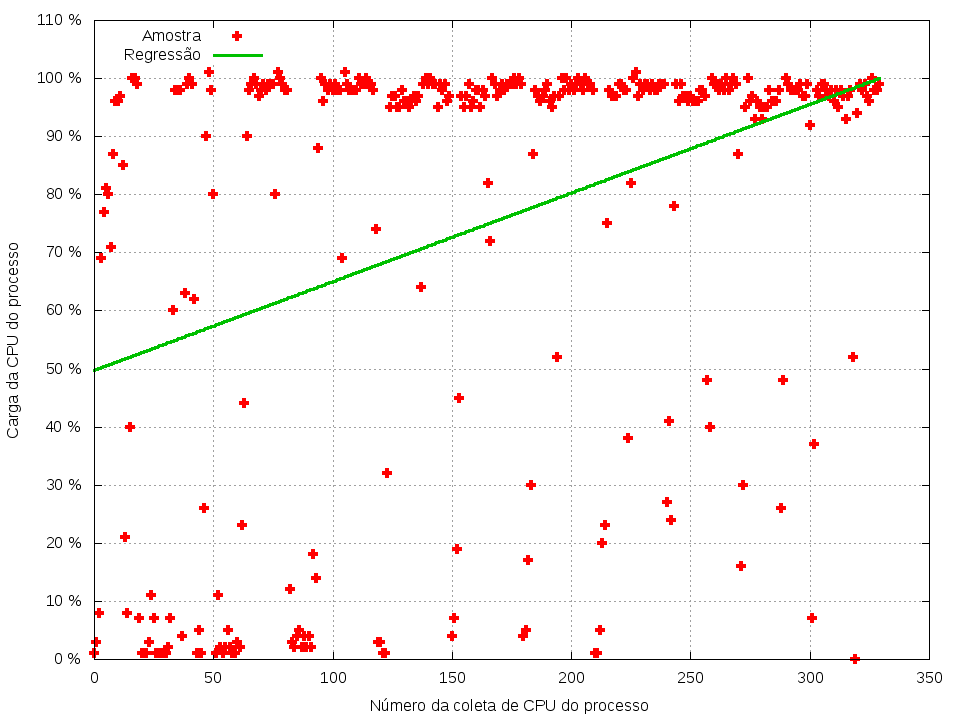
\includegraphics[width=\linewidth]{img/scatter-usr-cpu}
    \caption{Regressão linear da utilização de CPU do processo do controlador
    em função do número de coletas de CPU realizadas à medida que a rede 
    crescia}
\end{figure}

A reta representada pela regressão mostra o quão crescente é a utilização de 
CPU pelo processo à medida que a rede cresce.


\subsection{Consumo do controlador em relação ao sistema operacional}

Para computar um rede com 550 computadores o controlador utilizou 10\% da 
CPU do sistema operacional.
Como pode ser visto na figura \ref{fig:sys-cpu-growth} o crescimento da 
função de utilização de CPU do sistema é praticamente linear.
À medida que a rede cresce, os processadores do computador do controlador 
aumentam sua carga.

\begin{figure}[!htb]
    \centering
    \label{fig:sys-cpu-growth}
    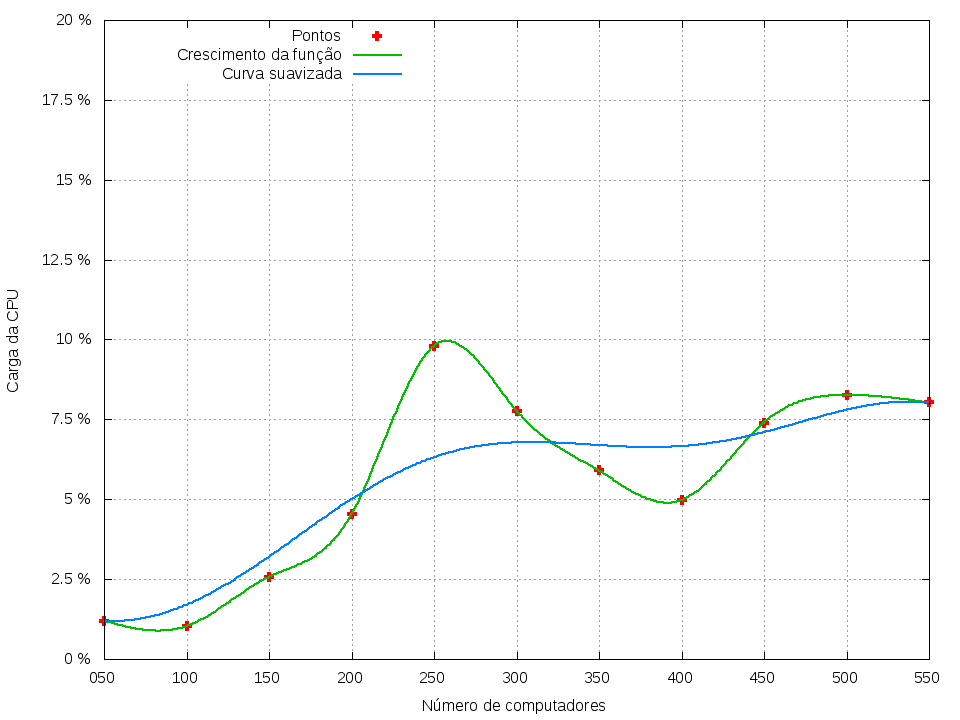
\includegraphics[width=\linewidth]{img/sys-cpu-growth}
    \caption{Crescimento da função de utilização da CPU do sistema operacional
    em função do crescimento de computadores na rede}
\end{figure}

O controlador POX é escrito na linguagem de programação \emph{Python}.
Cada nova entidade (computador ou comutador) ao ser detectado pelo controlador
recebe um identificador único.
Essas entidades são armazenadas em um dicionário \emph{Python}.
O dicionário é uma estrutura de dados primitiva da linguagem que implementa
uma tabela \emph{hash} \citep{maurer1975hash}.
Em função disso, para a computação do experimento temos que a complexidade 
de tempo é na ordem de $O(n)$ conforme mostrado a seguir.

As operações de adição, remoção e busca em tabelas \emph{hash} tem, no 
caso médio, custo constante na ordem de $O(1)$.
Assim, considerando-se $n$ o número de vértices, temos que para cada 
vértice do grafo o custo para inserí-lo durante o experimento é $O(1)$.
A complexidade de tempo do experimento, à medida que a rede cresce, é na 
ordem de $O(n)$.

Uma regressão linear foi computada da amostra coletada da carga de \emph{CPU}
do sistema operacional durante o experimento. 
A figura \ref{fig:scatter-sys-cpu} apresenta o resultado da regressão.

\begin{figure}[!htb]
    \centering
    \label{fig:scatter-sys-cpu}
    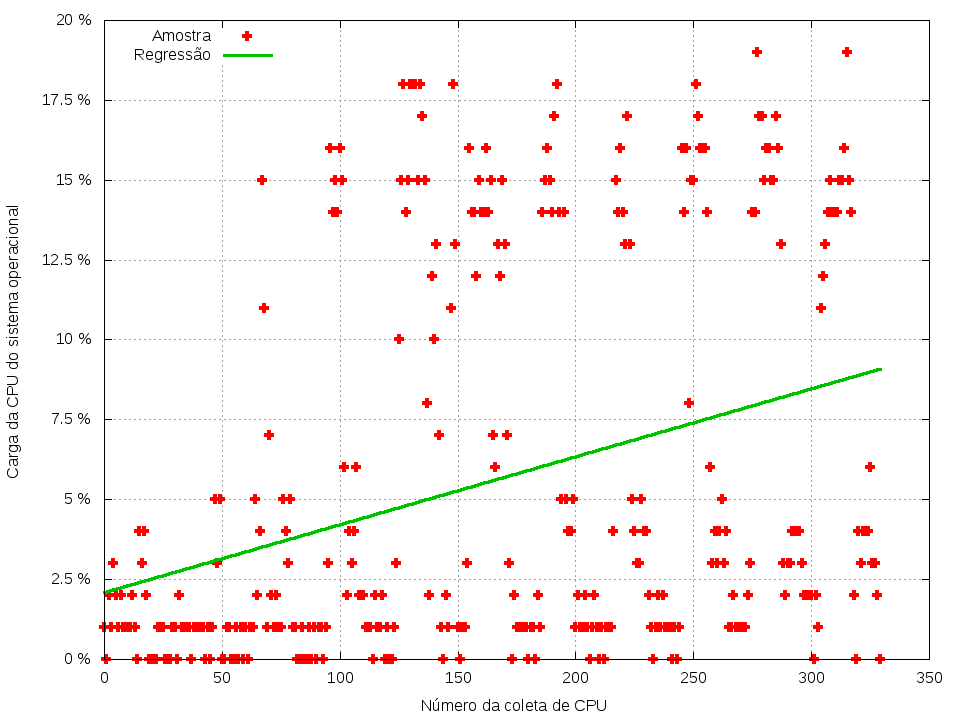
\includegraphics[width=\linewidth]{img/scatter-sys-cpu}
    \caption{Regressão linear sobre a carga de CPU do sistema operacional}
\end{figure}


\subsection{Consumo de memória}

A figura \ref{fig:memory-usage-growth} apresenta o crescimento da utilização
de memória à medida que a rede cresce. 
O computador do controlador possui 8 \emph{Gigabytes} de memória RAN 
(\emph{random access memory}). 
O consumo de memória pelo controlador durante o experimento variou de 2\% a 4\%
da memória global do sistema operacional.

O módulo \emph{Graph} adiciona vértices para cada computador e comutador 
identificados na rede.
Cada vértice é um objeto da classe \emph{Vertex}.
Esse objeto contém a referência para objetos das classes \emph{Host} e 
\emph{Switch} da entidade (computador ou comutador) que é representada pelo
vértice.
Assim, à medida que vértices são adicionados à rede, novos objetos são 
criados.
As arestas são objetos da classe \emph{Edge} e guardam referências para 
os objetos dos vértices que compõem a aresta.

\break
\begin{figure}[!htb]
    \centering
    \label{fig:memory-usage-growth}
    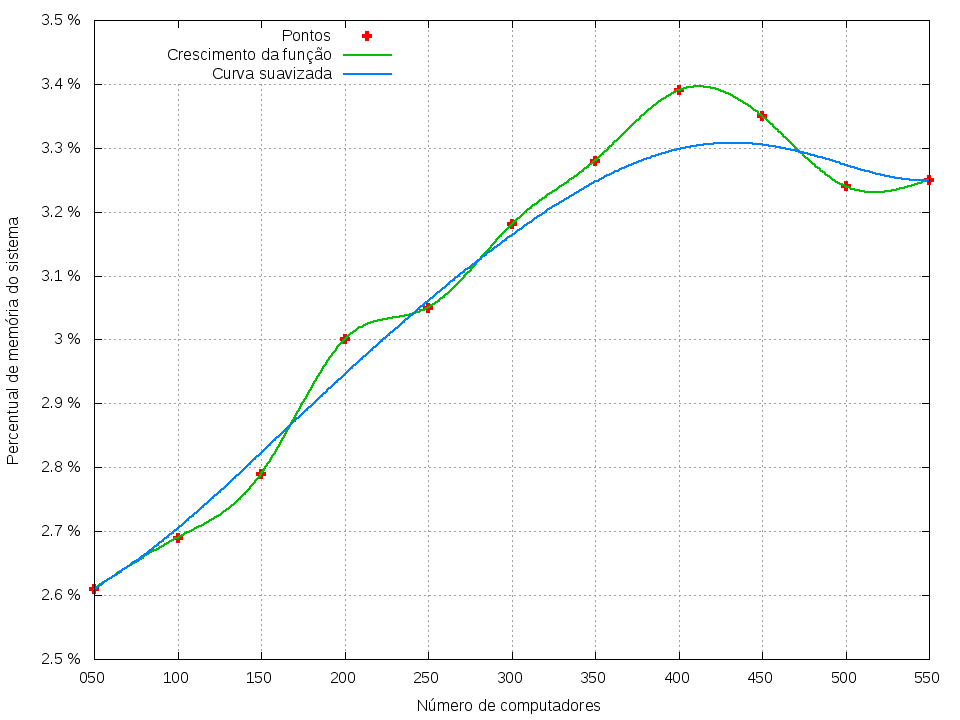
\includegraphics[width=\linewidth]{img/memory-usage-growth}
    \caption{Crescimento do percentual de utilização de memória pelo
    controlador à medida que o número de computadores na rede aumenta}
\end{figure}

Em função disso, assumiu-se que: Um objeto \emph{Vertex} ocupa na memória um 
espaço de endereçamento de tamanho $x$. 
E um objeto \emph{Edge} ocupa $y$.
Considerando-se $n$ o número de vértices e $m$ o número de arestas do grafo,
temos que a função que representa a utilização de memória (complexidade de 
espaço) é $nx + my$.
Ou seja, o número de vértices no grafo multiplicado pelo tamanho de um 
objeto de vértice na memória somado ao número de arestas do grafo 
multiplicado pelo tamanho de um objeto de aresta na memória.


A função de complexidade de espaço $nx + my$ mostra que o crescimento de 
utilização de memória do computador é dada em função do aumento de vértices
e arestas na rede.
No experimento executado, o número de vértices (coeficiente $n$) cresceu 
linearmente.
A regressão linear computada mostra o crescimento na utilização de memória 
pelo controlador à medida que mais computadores foram inseridos na rede ao 
longo da amostragem.
A figura \ref{fig:scatter-memory-usage} apresenta o resultado dessa 
computação.

\begin{figure}[!htb]
    \centering
    \label{fig:scatter-memory-usage}
    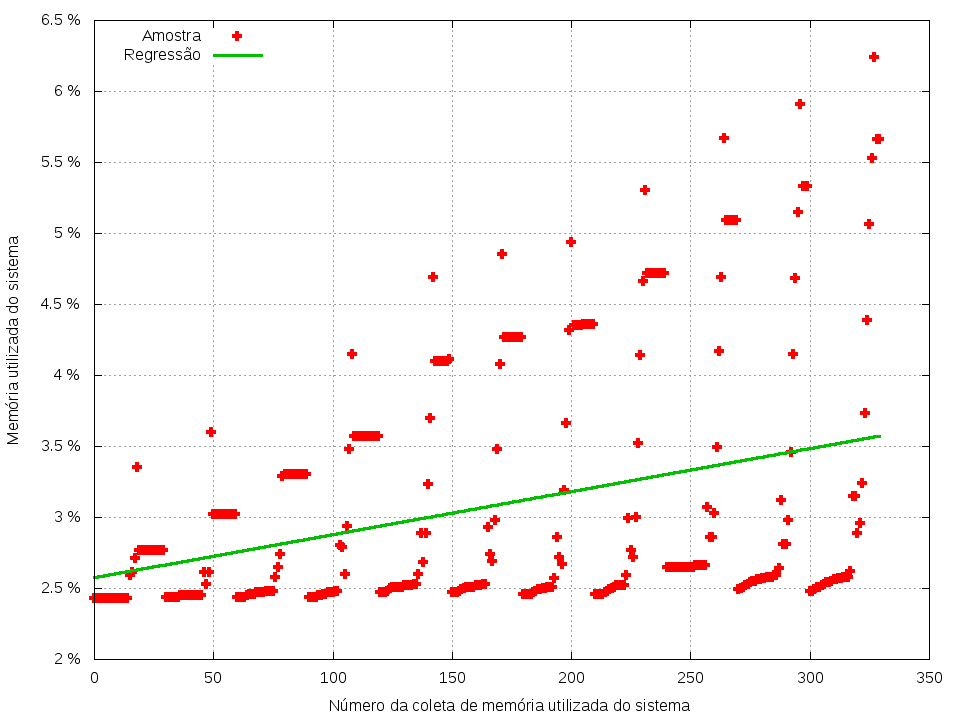
\includegraphics[width=\linewidth]{img/scatter-memory-usage}
    \caption{Regressão linear da amostra do consumo de memória do sistema
    à medida que rede cresce}
\end{figure}


\subsection{Taxa de escrita em memória secundária}

O módulo \emph{Graph} periodicamente salva uma imagem em memória secundária
com a visualização do grafo.
Durante o experimento de avaliação do controlador foi coletada a taxa de
escrita em disco à medida que a rede crescia. 

Em média, a taxa de escrita foi de 2 \emph{Megabytes} ao longo de cada 
iteração do experimento.
Para o experimento, uma imagem era gravada a cada 25 segundos.
Em cada iteração, mais vértices haviam no grafo, logo, mais objetos a serem 
mapeados na imagem. 

\break

Na figura \ref{fig:writing-rate-growth} é possível ver o crescimento na 
taxa de escrita em memória secundária à medida que a rede crescia.
Os pontos em vermelho representam os valores máximos de escrita coletados 
em cada iteração do experimento.
Uma interpolação passando por todos os pontos é dada pela curva de coloração
verde.
Uma suavização da curva de interpolação é traçada na cor azul mostrando 
o crescimento da taxa de escrita à medida que novos vértices vão sendo criados
durante as iterações do experimento.

\begin{figure}[!htb]
    \centering
    \label{fig:writing-rate-growth}
    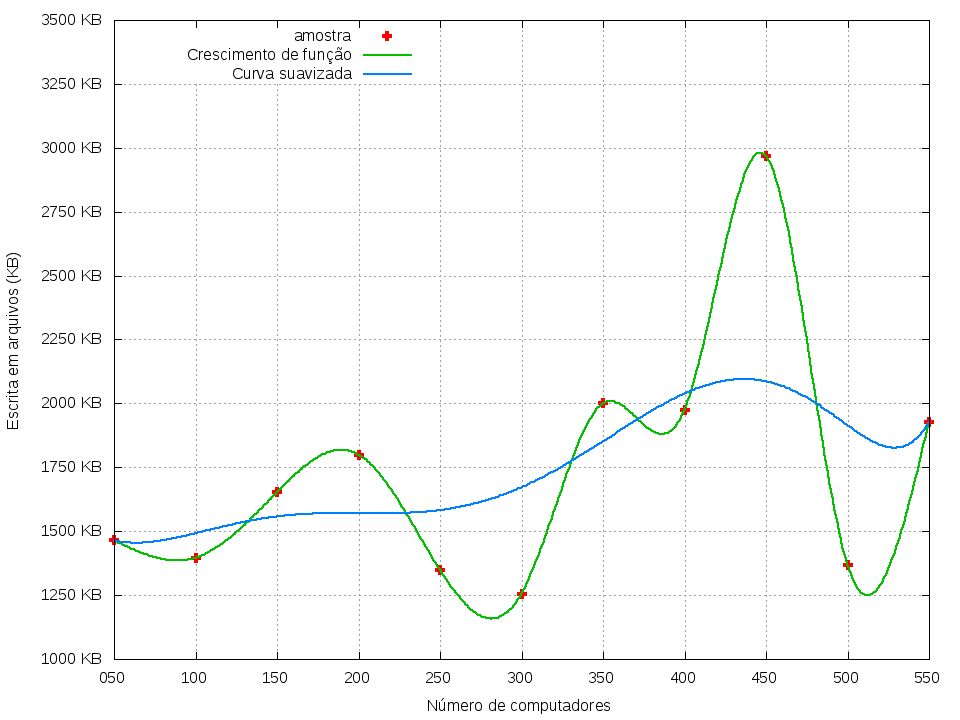
\includegraphics[width=\linewidth]{img/writing-rate-growth}
    \caption{Taxa de escrita em memória secundária à medida que a rede cresce}
\end{figure}

Uma regressão linear foi computada na amostra coletada das taxas de escrita
em memória secundária ao longo do experimento.
A figura \ref{fig:scatter-writing-rate} apresenta o resultado dessa regressão
mostrando o crescimento e a correlação entre os valores amostrados.

\begin{figure}[!htb]
    \centering
    \label{fig:scatter-writing-rate}
    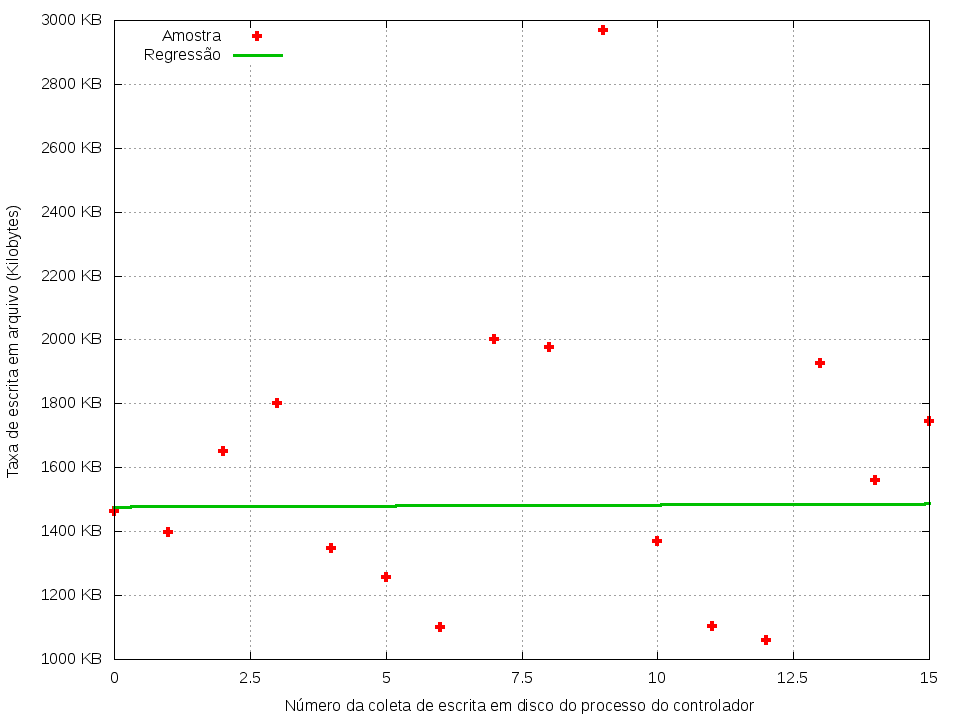
\includegraphics[width=\linewidth]{img/scatter-writing-rate}
    \caption{Regressão linear dos valores coletados da taxa de escrita em 
    memória secundária}
\end{figure}

\break
\section{Avaliação do módulo \emph{host\_tracker}}

O módulo \emph{host\_tracker} periodicamente envia pacotes \emph{APPPings} de
sondagem aos computadores da rede. 
Esta seção avalia o impacto e comportamento desse módulo em relação a rede e 
a solução.

Primeiramente é avaliada a largura de banda da rede e o impacto da sondagem 
de computadores nessa propriedade.
Em seguida a proporção de pacotes manipulados pelo controlador é comparada
em relação a quantidade de pacotes de sondagem.

\subsection{Avaliação de largura de banda}

Para medir a largura de banda foi utilizada a ferramenta de linha comando
\emph{iperf}.
A rede Ipê foi simulada com o conjunto completo de computadores.
6 pares de clientes e servidores \emph{iperf} foram executados durante 300 
segundos.
Cada par de cliente e servidor foi instanciado em máquinas virtuais 
diferentes e físicamente separadas.

\begin{table}[h!]
    \centering
    \begin{tabular}{ | l | l | l | l |}
    \hline
    \textbf{Teste} & \textbf{pingLim} & \textbf{entryMove} &
    \textbf{arpReply} \\ 
    \hline
    \hline Teste 0 & 5 & 50 & 5 \\ 
    \hline Teste 1 & 4 & 40 & 4 \\ 
    \hline Teste 2 & 3 & 30 & 3 \\ 
    \hline Teste 3 & 2 & 20 & 2 \\
    \hline Teste 4 & 1 & 10 & 1 \\
    \hline
    \end{tabular}
    \caption{Tabela com a relação de parâmetros por teste}
    \label{tbl:host_tracker-experiment}
\end{table}


Foram executados 5 baterias de testes.
Cada teste variou 3 parâmetro do módulo \emph{host\_tracker}.
O parâmetro \emph{pingLim} representa a quantidade de pacotes de sondagem 
necessários para considerar que um computador está inativo.
O parâmetro \emph{entryMove} é o tempo até que uma entrada do dicionário de 
endereços MAC seja alterado.
E o parâmetro \emph{arpReply} é o tempo a ser esperado pela resposta ARP até
que uma nova tentativa de sondagem seja enviada.
A tabela \ref{tbl:host_tracker-experiment} mostra de maneira resumida os 
experimentos executados.

\begin{figure}[!htb]
    \centering
    \label{fig:host_tracker-bandwidth}
    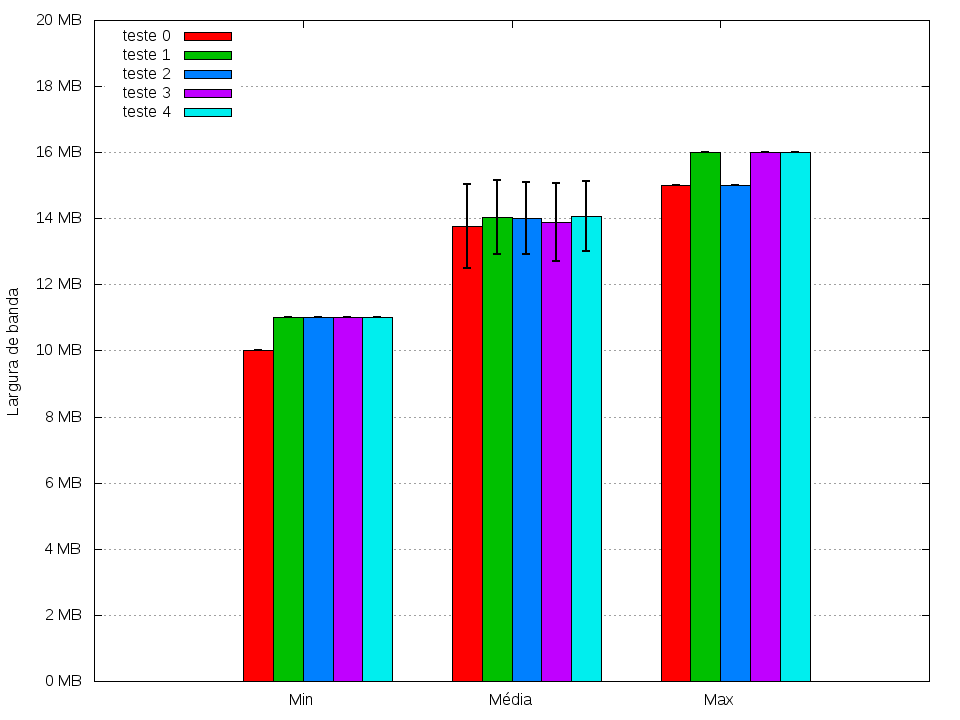
\includegraphics[width=\linewidth]{img/host_tracker-bandwidth}
    \caption{Largura de banda mínima, média com intervalo de confiança e máxima
    coletada da execução de cada teste do experimento}
\end{figure}

Para cada teste, durante 300 segundos, a cada 5 segundos a largura de banda
foi coletada.
A figura \ref{fig:host_tracker-bandwidth} mostra os valores mínimos, médio 
com intervalo de confiança e máximo da largura de banda coletada nos testes.

Como existiam 6 pares de clientes e servidores, a largura de banda é 
dividida entre esses computadores.
A média foi computada do somatório da largura de banda computada por cada 
par de cliente e servidor.

Conforme visto na tabela \ref{tbl:host_tracker-experiment} do Teste 0 ao 
Teste 4 os parâmetros avaliados foram decrementados. 
Em função disso, à medida que os testes foram executados nessa ordem, 
o intervalo de sondagem, o tempo de expiração e o tempo de aguardo por 
resposta reduziram. 
Essa redução faz com que a cada iteração de testes mais pacotes de sondagem
fossem disseminados na rede.
A figura \ref{fig:host_tracker-bandwidth} mostra que, apesar do aumento de 
pacotes de sondagem, a largura de banda média da rede não sofreu impacto 
considerável.
A figura \ref{fig:host_tracker-bandwidth-growth} apresenta a curva de 
interpolação entre os pontos representando a largura de banda média em cada 
teste do experimento.

\begin{figure}[!htb]
    \centering
    \label{fig:host_tracker-bandwidth-growth}
    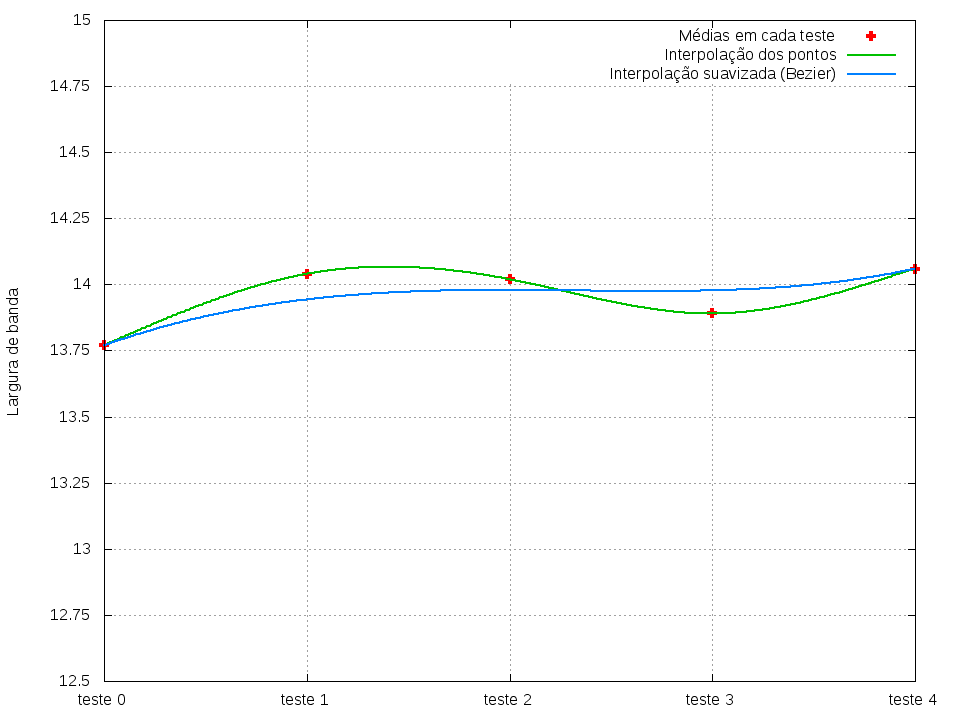
\includegraphics[width=\linewidth]{img/host_tracker-bandwidth-growth}
    \caption{Curva de interpolação das médias das larguras de banda medidas 
    em teste do experimento}
\end{figure}

\subsection{Avaliação do número de pacotes}

Essa subseção avalia a quantidade de pacotes de sondagem disparadas pelo 
módulo \emph{host\_tracker} à medida que mais computadores estão presentes
na rede.
São avaliados também, a quantidade de pacotes de entrada (\emph{PacketIn}) 
que o controlador lida à medida que a rede cresce.

O experimento começou com 50 computadores na rede.
Em cada iteração, novos 50 computadores foram adicionados à rede.
Ao final, a rede Ipê simulada, possuía 550 computadores.
Para computar o número de pacotes de sondagem foi adicionado um contador 
na funçao que envia esses pacotes.
A figura \ref{fig:npings} mostra o gráfico resultante dos valores computados
dos número de pacotes de sondagem enviados à medida que mais computadores 
estavam presentes na rede.

\begin{figure}[!htb]
    \centering
    \label{fig:npings}
    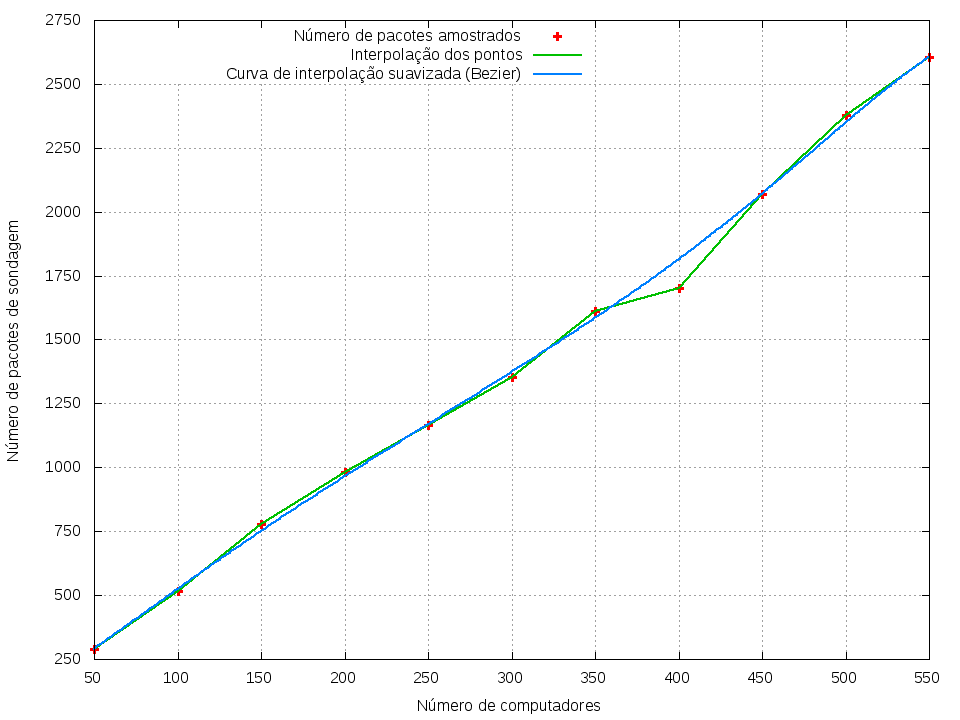
\includegraphics[width=\linewidth]{img/npings}
    \caption{Crescimento do número de pacotes de sondagens encaminhados 
        à medida que a rede crescia}
\end{figure}

O aumento do número de pacotes apresentou um crescimento linear.
Ou seja, à medida que mais computadores entram na rede, o número de pacotes
cresce na mesma proporção.
Para esse experimento, foi calculada a diferença da quantidade de pacotes da
iteração posterior com a iteração anterior.
Assim, é possível saber quantos pacotes variaram a cada iteração do 
experimento.
Esse resultado é apresentado na figura \ref{fig:npings-stats}. 

Em média, 200 a 250 pacotes a mais foram disparados a cada iteração. 
O experimento durou, para cada iteração, dois minutos. 
Considerando esse intervalo de tempo e a média de pacotes enviados, pode-se 
dizer que aproximadamente 5 pacotes foram enviados para cada computador 
identificado pelo grafo.
Levando em conta a média de 250 pacotes por iteração e que cada iteração 
adiciona 50 novos computadores, temos que a razão desses valores mostra 
que, para cada computador, durante dois minutos foram enviados 5 pacotes 
de sondagem.

\begin{figure}[!htb]
    \centering
    \label{fig:npings-stats}
    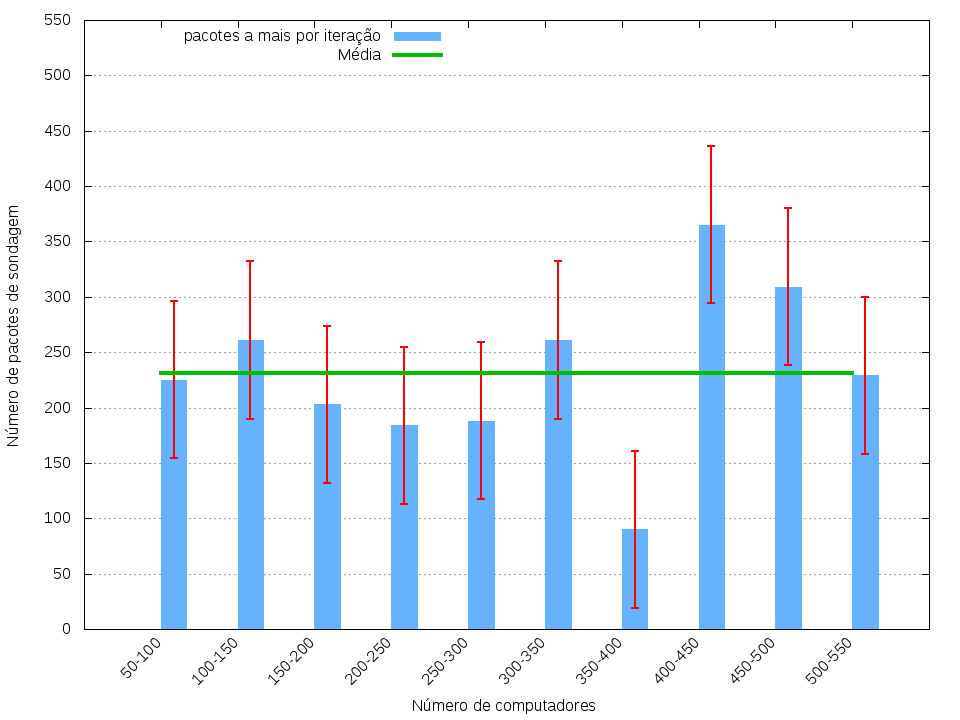
\includegraphics[width=\linewidth]{img/npings-stats}
    \caption{Diferença da quantidade de pacotes de sondagem enviados entre 
    cada par de iterações do experimento}
\end{figure}

O número de pacotes de entrada foi contabilizado contando as chamadas do 
evento \emph{PacketIn} no controlador.
Foram medidos quantos pacotes de entrada o controlador manipulava a cada 
iteração do experimento.

A figura \ref{fig:packets-in} mostra o crescimento no número de pacotes ao 
longo do experimento. 
Assim como o número de pacotes de sondagem, o número de pacotes 
(\emph{PacketIn}) cresce linearmente.
Ou seja, à medida que mais computares estão na rede, o volume de pacotes de 
entrada cresce proporcionalmente.

\begin{figure}[!htb]
    \centering
    \label{fig:packets-in}
    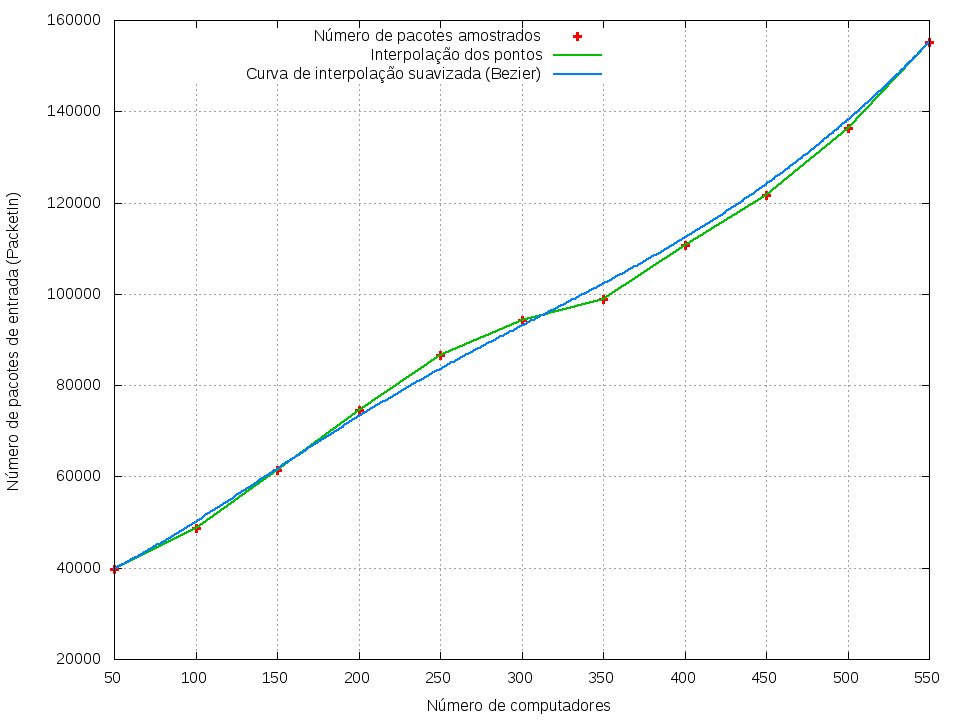
\includegraphics[width=\linewidth]{img/packets-in}
    \caption{Número de pacotes de entrada (\emph{PacketIn}) manipuladas pelo
    controlador em cada iteraçao do experimento}
\end{figure}


Para o experimento da contagem do número de pacotes de entrada no controlador
foram computadas as diferenças entre os experimentos posteriores e os
anteriores.
Em média doze mil pacotes de entrada foram manipulados a mais em cada 
iteração do experimento.

A figura \ref{fig:packets-in-stats} mostra os resultados desse experimento.
A linhas verticais vermelhas apresentam o intervalo de confiança dos valores
amostrados das diferenças. 
O erro padrão baixo prova o comportamento mostrado na figura 
\ref{fig:packets-in} sobre o crescimento linear no número de pacotes de 
entrada.

Considerando o intervalo de tempo de dois minutos de execução do experimento e 
que, a cada iteração cinquenta novos computadores foram adicionados, 
tem-se que a razão da média pelo número de computadores por iteração é igual 
a 250 pacotes. 
O controlador lida com pacotes que nem sempre são originados de computadores.
Assim, esse valor calculado é apenas uma aproximação do número de pacotes 
que o controlador manipula em função do número de computadores.

\begin{figure}[!htb]
    \centering
    \label{fig:packets-in-stats}
    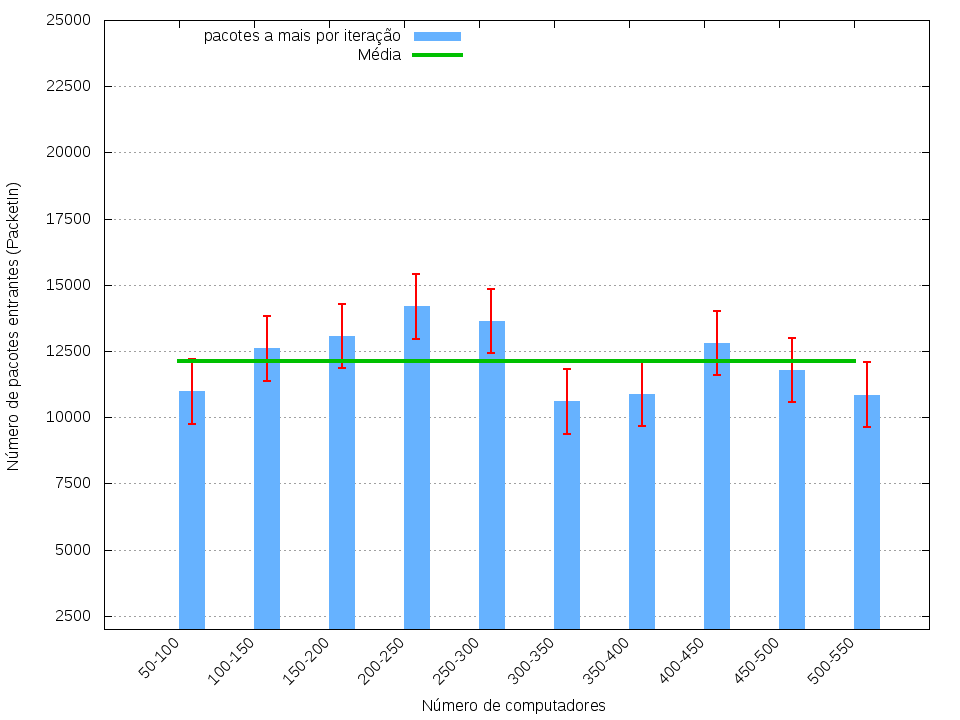
\includegraphics[width=\linewidth]{img/packets-in-stats}
    \caption{Diferença da quantidade de pacotes de entrada (\emph{PacketIn})
    manipuladas no controlador entre cada par de iterações do experimento}
\end{figure}

\subsection{Comparação dos números de pacotes}

Essa subseção compara o número de pacotes de sondagem com o número de pacotes
de entrada que o controlador lida.
A comparação é feita em quantidade e em percentual.
A seguir serão apresentados os resultados dessa avaliação.

A comparação do número de pacotes é mostrada na figura
\ref{fig:npings-x-packets-in}.
Os valores nas coordenadas $y$ (ordenadas) estão em escala exponencial, o que 
facilita a visualização da diferença entre o número de pacotes de entrada
(\emph{PacketIn}) e pacotes de sondagem.

Com a rede Ipê simulada completa foram enviados, no máximo, quase $3$ mil 
pacotes de sondagem e quase $150.000$ pacotes de entrada manipulados pelo 
controlador.
\break
\begin{figure}[!htb]
    \centering
    \label{fig:npings-x-packets-in}
    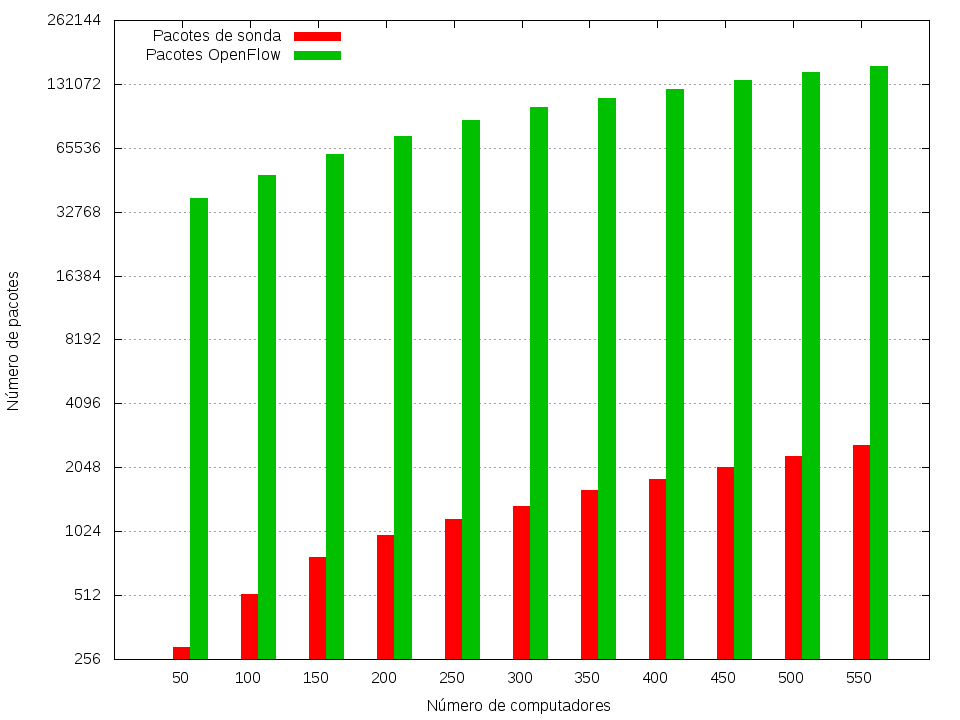
\includegraphics[width=\linewidth]{img/npings-x-packets-in}
    \caption{Comparação do número de pacotes de sondagem e de entrada 
    manipulados pelo controlador}
\end{figure}

O total de pacotes manipulados pelo controlador é representado pela soma 
do número total de pacotes de sondagem com o número total de pacotes de 
entrada (\emph{PacketIn}).
Em função disso a figura \ref{fig:npings-x-packets-in-stacked} apresenta 
as proporções em percentuais dos dois tipos de pacotes.

Nas abscissas tem-se o número de computadores na rede a cada iteração do 
experimento.
Nas ordenadas tem-se os percentuais do número total de pacotes manipulados 
pelo controlador.
É possível notar que os pacotes de sondagem representam um percentual muito 
baixo em relação ao total de pacotes.

Como apresentado na subseção de avaliação da largura de banda em função do 
módulo \emph{host\_tracker}, os pacotes de sondagem não causam muito impacto 
no funcionamento da rede e não representam um grande volume de pacotes.
Para o presente experimento esses pacotes, em seu pior caso, representaram
$2\%$ do total de pacotes manipulados pelo controlador.

\begin{figure}[!htb]
    \centering
    \label{fig:npings-x-packets-in-stacked}
    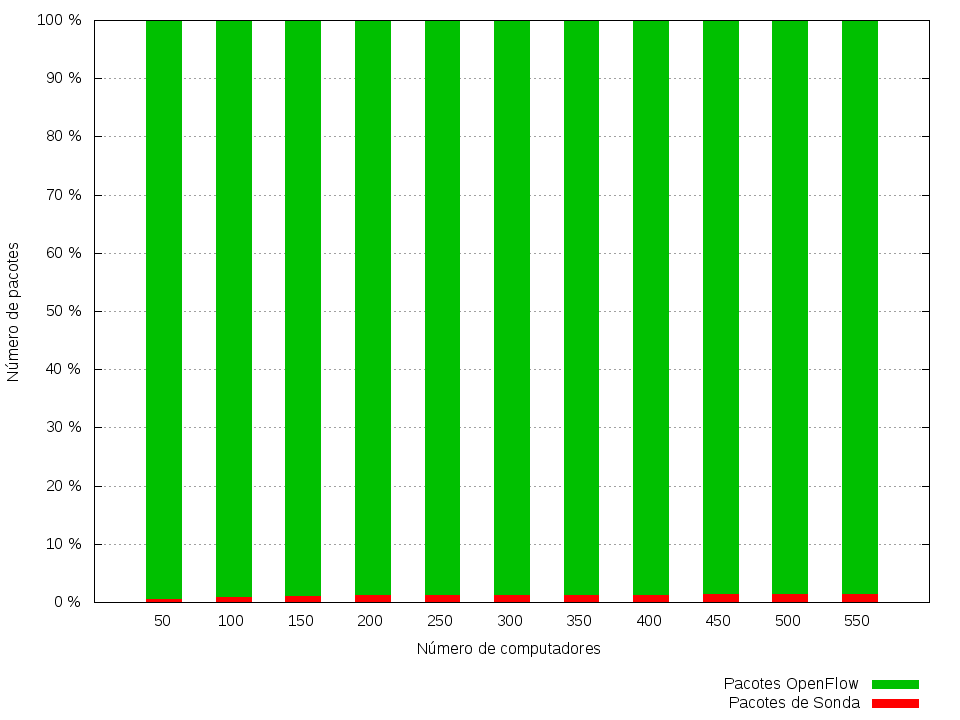
\includegraphics[width=\linewidth]{img/npings-x-packets-in-stacked}
    \caption{Valores percentuais do número de pacotes de sondagem e de 
        entrada manipulados pelo controlador}
\end{figure}

\section{Avaliação da rede}

Nesta seção são avaliados latência, largura de banda e \emph{jitter} da 
rede Ipê simulada.
Para cada cenário avaliado foram feitas comparações com e sem a presença 
do controlador com a solução em grafos. 
É avaliado o impacto da solução em grafos na rede.

\subsection{Avaliação de latência}

Em função do ambiente virtualizado, o experimento de latência foi dividido em 
duas partes.
A primeira avaliou a latência das redes locais.
Ou seja, a latência entre computadores de uma mesma subrede dentro de uma 
máquina virtual.
A segunda parte, avaliou a latência da rede global.
Ou seja, entre servidor físicos diferentes, fazendo com que os pacotes 
passem por toda a infraestrutura física do ambiente de simulação.
Para cada caso, foram medidos a latência com e sem o controlador em grafos.

Com a rede Ipê simulada completa foram executados, simultaneamente, 
6 pares de computadores enviando pacotes de ICMP PING. 
As medições da latência foram coletadas a cada segundo da execução do 
experimento. 
A latência em cada instante é a média de todos os 6 pares de computadores
a cada iteração de coleta.

\subsubsection{Latência da rede local}

A figura \ref{fig:local-latency} mostra a latência medida ao longo do 
experimento para as redes locais.
É possível notar que a latência da solução com controlador, no início do 
experimento, está em torno de 4 milisegundos.
Esse valor ocorre em função do encaminhamento, pelo comutador, do primeiro 
pacote para o controlador. 
Os valores subsequentes são próximos ao valor da latência medido na solução 
sem controlador.

\begin{figure}[!htb]
    \centering
    \label{fig:local-latency}
    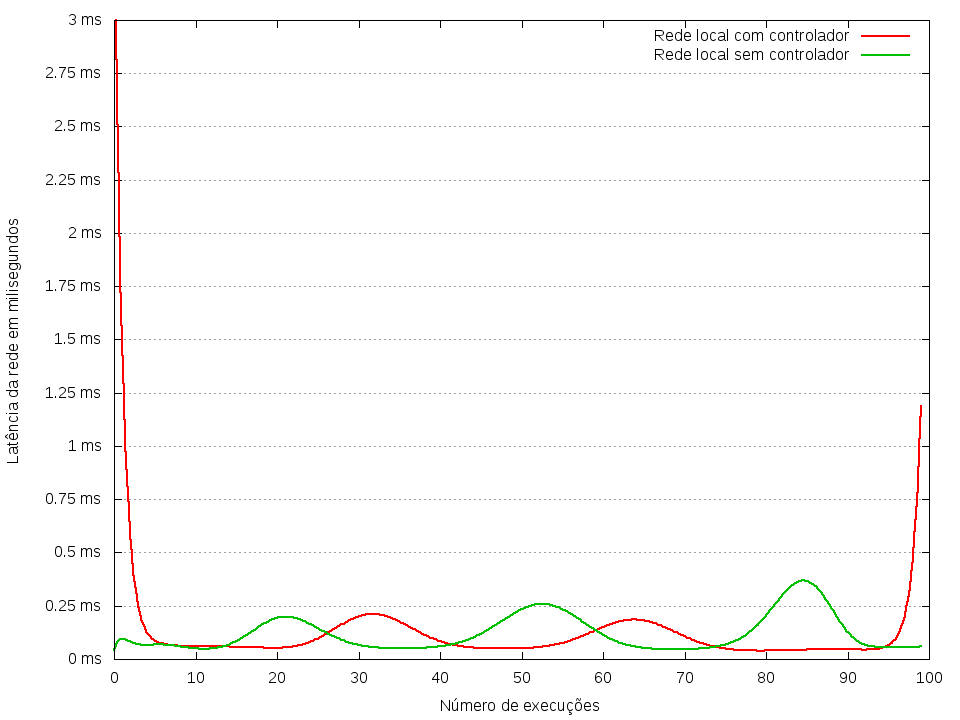
\includegraphics[width=\linewidth]{img/local-latency}
    \caption{Latência média das redes locais com e sem o controlador com a 
    solução em grafos}
\end{figure}

Uma avaliação dos dados coletados da largura de banda no ambiente das 
redes locais foi realizada.
Os valores de latência mínima, máxima e média com intervalo de confiança 
são apresentados na figura \ref{fig:local-latency-stats}.
No geral, as latências da rede com a solução do controlador em grafos e 
sem controlador se mantiveram parecidas. 
Em média, a latência no experimento das redes locais foi de 
$0,13$ milisegundos.
É possível notar através do intervalo de confiança que a latência na rede 
com o controlador se manteve mais constante ao longo do experimento.
Ou seja, mais confiável, com baixa variancia.

\begin{figure}[!htb]
    \centering
    \label{fig:local-latency-stats}
    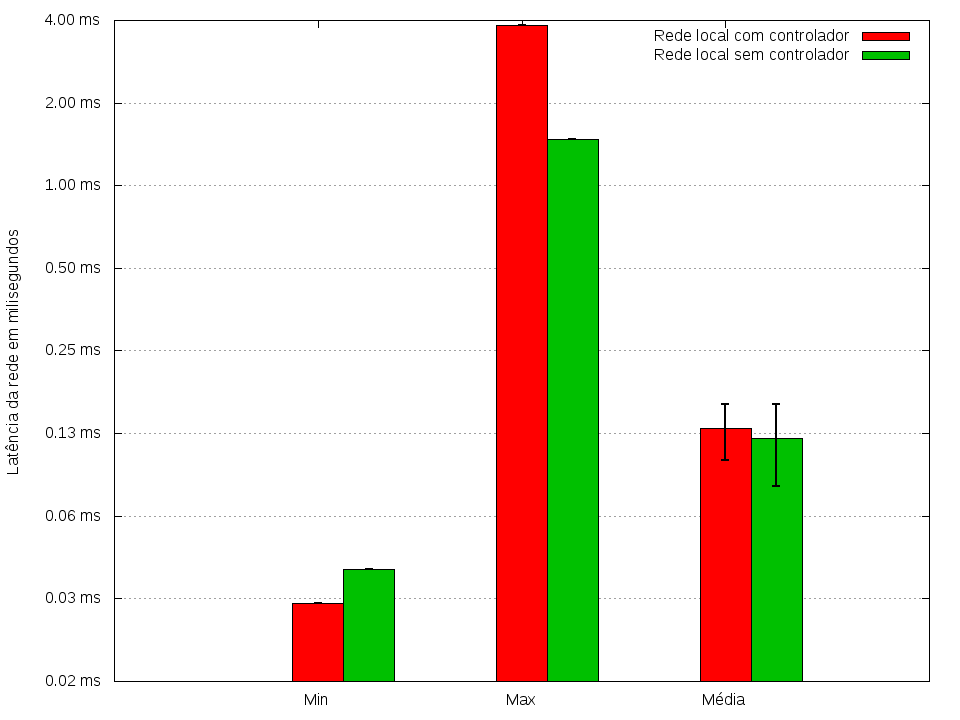
\includegraphics[width=\linewidth]{img/local-latency-stats}
    \caption{Latência mínima, máxima e média das redes locais}
\end{figure}


\subsubsection{Latência da rede global Ipê}

O mesmo perfil de experimento foi executado para o cenário da rede global.
6 pares de computadores executaram PINGs coletando os valores da latência
a cada segundo.
Para esse experimento, foram separados os pares em computadores diferentes 
para garantir que cada pacote trafegasse por toda infraestrutura física da 
rede simulada. 

A figura \ref{fig:ipe-latency} apresenta os resultados dessa avaliação.
Como pode ser visto, a latência inicial coletada na rede com a solução do 
controlador com o módulo grafo chegou a 400 milisegundos.
Esse valor ocorre em função do primeiro pacotes que é encaminhado para o 
controlador.
No geral, a latência da rede sem controlador sofreu uma variação mais alta.
Em contraponto a curva da latência com o controlador demonstra-se mais 
constante.

\begin{figure}[!htb]
    \centering
    \label{fig:ipe-latency}
    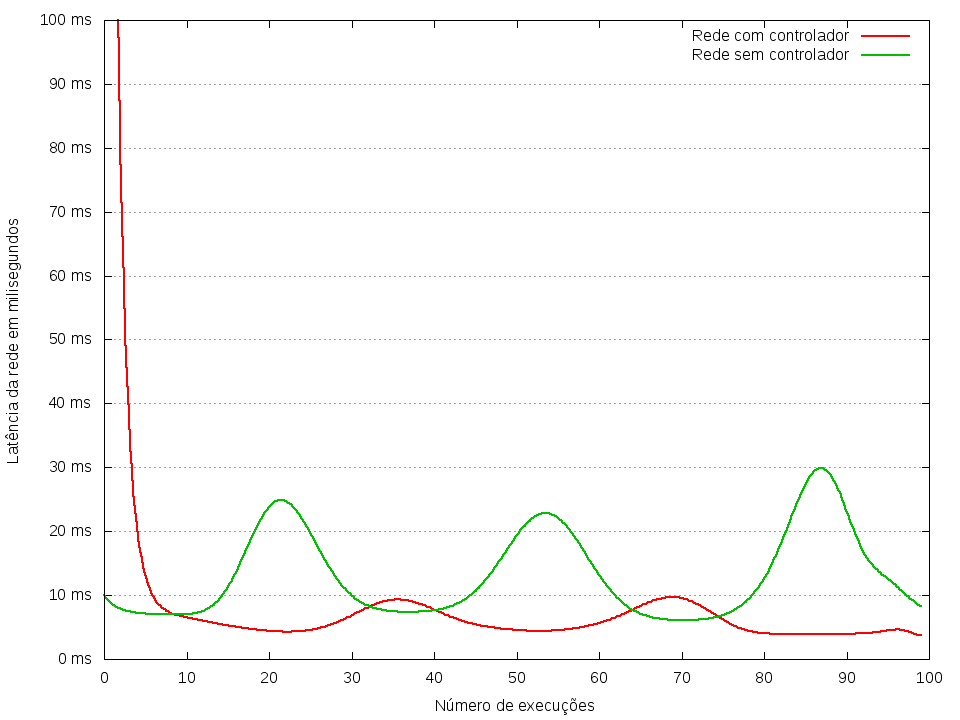
\includegraphics[width=\linewidth]{img/ipe-latency}
    \caption{Latência da rede Ipê com e sem o controlador com a solução em 
    grafos}
\end{figure}

Em média, a latência da rede Ipê simulada foi $13$ milisegundos.
Na rede global, o experimento sem controlador teve oscilações bem altas que
chegaram a valores de $100$ milisegundos de latência.
É possível notar novamente a estabilidade da rede com controlador observando
o desvio padrão mais baixo. 
A figura \ref{fig:ipe-latency-stats} apresenta os resultados da avaliação dos
valores mínimos, máximos e médios com desvio padrão da rede Ipê simulada.

Através dos experimento de latência realizados tanto nas redes locais quanto 
na rede Ipê global, pode-se notar que o controlador com a solução do módulo 
em grafos não gerou grande impacto na rede.
Com exceção dos primeiros pacotes, com uma latência alta, a rede com o 
controlador se mostrou mais estável do que sem. 

\begin{figure}[!htb]
    \centering
    \label{fig:ipe-latency-stats}
    \includegraphics[width=\linewidth]{img/ipe-latency-stats}
    \caption{Avaliação da latência da rede Ipê considerando os valores mínimos,
    máximos e médios analisados}
\end{figure}

\subsection{Avaliação de largura de banda}

A avaliação da largura de banda foi feita utilizando 4 pares de computadores
em subredes e serivodores da rede física diferentes.
Para cada par de computadores, foi utilizada a ferramenta de linha comando
\emph{iperf}.
O experimento consistiu em medir, com intervalos de 5 segundos, durante 
5 minutos, a largura de banda através de conexões TCP.
A largura de banda medida é representada pela média das quatro medições a
cada iteração de coleta durante o experimento.

A largura de banda da rede sem controlador medida durante o experimento foi, 
em média, $18$ \emph{Megabytes}.
Na figura \ref{fig:bandwidth-no-ctrl} são apresentados os resultados do 
experimento. 
Conforme pode ser visto nesta figura, os pontos representam os valores 
médios amostrados em todos os pares de computadores que estavam coletando 
a largura de banda.
Uma interpolação suavizada e uma passando por todos os pontos médios mostram
a largura de banda média computada nesse experimento.

\begin{figure}[!htb]
    \centering
    \label{fig:bandwidth-no-ctrl}
    \includegraphics[width=\linewidth]{img/bandwidth-no-ctrl}
    \caption{Largura de banda média da rede sem controlador}
\end{figure}


\subsection{Avaliação de \emph{jitter}}


\subsection{Avaliação de percentual de erros}





%\chapter{Aplicações}


\section{Árvore geradora mínima}

\section{Caminho mínimo}

\section{Balanceamento de carga}

%\chapter{Análise}

\section{Complexidade de Tempo}

\section{Complexidade de Espaço}

%\chapter{Trabalhos futuros}
\label{chap:future-work}

Como uma proposta futura, criar visualizador em tempo real do grafo que 
interaja com o administrador da rede e mostre, de uma maneira simples, 
toda a operação da rede.

Assim como o controlador POX, o módulo proposto, ao ter seu processo terminado,
não persiste as informações de estado da rede.
Todo o grafo computado é perdido.
Em função disso, um banco de dados em grafos, distribuído, poderia ser 
utilizado para persistir o grafo, e as informações do estado da rede, de 
maneira confiável e tolerante a falhas. 

Algoritmos genéricos em grafos poderiam ser implementados como uma biblioteca
para o módulo.
Assim, estabelecida uma periodicidade, esses algoritmos poderiam ser computados
no grafo e seus resultados publicados como extensão da API.

\section{Conclusão}

\begin{frame}{Conclusão}

\end{frame}



% Bibliograph file
\ppgccbibliography{src/references}


%\input{apendice} % ARQUIVO CONTENDO OS APÊNDICES : OPCIONAL
%\input{anexo} % ARQUIVO CONTENDO OS ANEXOS: OPCIONAL

\end{document}
